\documentclass[12pt,american]{paper}

\usepackage[T1]{fontenc}
\usepackage[latin9]{inputenc}
\usepackage[margin=1.5in]{geometry}
\usepackage{graphics}
\geometry{verbose}
%\usepackage[monochrome]{color} %no colors
\usepackage{color} %with color
\usepackage{textcomp}
\usepackage{amsthm,amssymb,amsmath}
\usepackage{enumerate}
\usepackage{graphicx}
\usepackage{setspace} 
\usepackage{courier}
\usepackage{hyperref}
\usepackage{url}
\usepackage[authoryear]{natbib} 
\usepackage{subfig}
\usepackage{caption}
%\usepackage{subcaption} %cannot be used with subfig package
\usepackage[normalem]{ulem}
\usepackage{bbm}
\usepackage{rotating}

\newcommand\hcancel[2][black]{\setbox0=\hbox{$#2$}%
\rlap{\raisebox{.45\ht0}{\textcolor{#1}{\rule{\wd0}{1pt}}}}#2} 

%\usepackage[colorinlistoftodos, obeyDraft]{todonotes} % no todo's
\usepackage[colorinlistoftodos]{todonotes} % with todo's
\onehalfspacing

%\usepackage[percent]{overpic}


\usepackage{tikz}
\usetikzlibrary{calc}
\colorlet{examplefill}{blue!10}

\newcommand{\tikzmark}[1]{\tikz[overlay,remember picture] \node (#1) {};}
\newcommand{\DrawBox}[1][]{%
    \tikz[overlay,remember picture]{
    \draw[red,#1]
      ($(left)+(-0.2em,0.9em)$) rectangle
      ($(right)+(0.2em,-0.3em)$);}
}
%\makeatletter

%%%%%%%%%%%%%%%%%%%%%%%%%%%%%% Textclass specific LaTeX commands.
\theoremstyle{remark} 
\newtheorem*{acknowledgement*}{\protect\acknowledgementname} \theoremstyle{plain} 
\newtheorem{thm}{\protect\theoremname} \theoremstyle{plain} 
\newtheorem{prop}{Proposition}
\newtheorem{ass}{Assumption}
\newtheorem{lemma}{Lemma}
\newtheorem{ex}{Example}
\newtheorem{remark}{Remark}
\newtheorem{cor}{Corollary}

\makeatother
\usepackage{babel} 
\providecommand{\acknowledgementname}{Acknowledgement} 
\providecommand{\lemmaname}{Lemma} 
\providecommand{\theoremname}{Theorem}

\begin{document}

\title{\vspace*{-3cm} Task Discretion, Labor Market Frictions and Entrepreneurship\footnote{This paper supersedes an earlier version titled ``The Value of Entrepreneurial Failures: Task Allocation and Career Concerns'' \citep{canidio2016}. We are grateful to Carlos Casso Dominguez for excellent research assistance. We are also grateful to Chris Avery, Raul Baptista, Werner B\"onte, Jing-Yuan Chiou, Roberta Dessi, Robert Gibbons, Denis Gromb, Thomas Hellmann, Andrea Mantovani, Massimo Riccaboni, Marko Tervi\"o, Peter Thompson, John van Reenen, Michael Waldman, Timothy van Zandt,  conference participants at the CEPR Workshop in Entrepreneurship Economics,  the Annual Searle Center Conference on Innovation Economics,  the 2018 ASSA meetings, the Organizational lunch workshop at MIT, the ZEW Conference on the Dynamics of Entrepreneurship, as well as seminar participants at the University of Montr\'eal, INSEAD, and HEC Paris. 
Legros gratefully acknowledges the financial support of the European Research Council under the European Union's Seventh Framework Programme (FP7/2007-2013 / ERC grant agreement n\textdegree 339950.)}
}
\author{Andrea Canidio\thanks{IMT School of Advanced Studies, Lucca; andrea.canidio@imtlucca.it}  and Patrick Legros\thanks{Universit\'e libre de Bruxelles (ECARES) and CEPR; Patrick.Legros@ulb.be.}}

\maketitle 

\noindent This version: \today

\begin{abstract}
\singlespacing
An agent can perform a job in several ways, which we call \textit{tasks}.  The decision rights over which task to choose change with the agent's occupation: it is the prerogative of management within firms, and of the agent himself if he is an entrepreneur. While an agent's comparative advantage at different tasks is unknown, it can be learned by observing his performance. However, tasks that generate more information may also lead to lower short-term expected profits. Hence in the presence of contracting frictions firms will allocate workers to more informative tasks only if workers cannot easily move to other firms. In this case, agents may prefer to become entrepreneurs and acquire task discretion, even if their short-term payoff is lower than in firms. The model generates novel predictions with respect to, for example, the payoff and wage dynamics of agents who switch between entrepreneurship and employment.

%Incompleteness of contracting together with labor-market frictions jointly determine a novel motive for entrepreneurship: acquiring discretion over task allocation. 


\end{abstract}
%\vspace{3mm}
%
\noindent \textbf{JEL classification:} D83, J24, J62, J63, L26, M13.\\
\noindent\textbf{Keywords} Task discretion, organizational choice, entrepreneurship, labor-market frictions, entrepreneurial failures, learning.



\pagebreak
\section{Introduction}
The property right literature  has long argued that contracting frictions may prevent the efficient allocation of inputs within production units \citep{Grossman1986}. An overlooked implication is that, to the extent that the allocation of residual decision rights differs  across occupations,  contractual frictions may  lead to misallocation of inputs also across occupations. Motivated by this observation, we study how contractual frictions affect both agents' sorting across occupation and then, within each production unit, between different ways to do a job, which we call \textit{tasks}.   We do so by building a two-period model in which agents first sort between employment in a firm and entrepreneurship, and then between one of two tasks. An agent's productivity at different tasks, i.e., his talent, is unknown but can be learned by observing his performance at a task, with some tasks being more informative than others. However, task allocation is not contractible. As in the property right literature, task allocation is chosen by owners or management within firms, and by the  agent himself if he is an entrepreneur. 

Examples of non contractible tasks informative about talent are plentiful. A contract with a scientist defines the objective of the research (e.g., find a cure for Alzheimer) but not the exact experimental design, even if the experimental design may reveal the scientist's comparative talent at following well established or unusual research paths. A contract with a new manager does not specify the exact organizational chart of the firm (people under his authority or people who have authority on him), and, as a consequence, does not specify the extent to which he can delegate or centralize decisions. Delegating or centralizing decisions may, however, reveal his comparative advantage at different styles of management.

An initial result is a novel motive for entrepreneurship: we show that an agent may become entrepreneur to gain task discretion and learn his talent. This motive resembles the  well-documented ``be one's own boss'' motive  (see for example the survey by \citealp{stephan2015understanding}). Importantly, however, we do not assume that individuals have an intrinsic benefit from task discretion, from being their own boss. Becoming an entrepreneur to acquire task discretion is beneficial if and only if learning is less than efficient within firms. This, in turns, depends on the level of labor market frictions which, in the model, are measured by the  probability that an agent receives an external wage offer. As this probability decreases, firms are more likely to allocate their  employees to informative tasks because they capture part of the benefit of learning their workers' comparative advantage.%\footnote{This is similar to  \cite{acemoglu1999structure}, in which as labor market frictions increase firms become more likely to invest in generic human capital. The novelty here is the study of how labor market frictions affects agents' occupational choices by determining whether learning is possible within firms.} 
It follows that agents are less likely to become entrepreneur to gain task discretion when labor market frictions are high. {\color{blue}Hence, the novelty here is to connect labor market frictions, with firms' internal organization, with agent's career choice.\footnote{That is, the connection between labor market frictions and organizational choice was noted before. For example, in \cite{acemoglu1999structure}, as labor market frictions increase firms become more likely to invest in generic human capital. Here we point out that these changes in organizational structure have implication for career choice.}}

A second contribution is to link the level of labor market fictions to the productivity of former entrepreneurs relative to former workers, hence to their respective wage dynamics. When labor market fictions are low, some agents will become entrepreneurs to learn their talents, which cannot happen within firms. As a consequence, in the following period, if these agents decide to switch occupation, they will earn a higher wage than former workers---there is a \textit{positive wage premium for former entrepreneur}. On the other hand, if labor market frictions are high, learning will occur within firms. Agents may choose entrepreneurship if they have a very valuable business idea or if they fail to find a job. These agents are less likely then workers to choose an informative task allocation, leading to a \textit{negative wage premium for former entrepreneurs}.%\footnote{Available empirical results show, indeed,  that the wage premium for former entrepreneurs can be both positive or negative. For example, \cite{hamilton2000does} finds a positive premium in the US. \cite{luzzi2016individual} also finds a positive premium in Norway. However, \cite*{baptista2012former} finds a negative premium in Portugal.}

The model therefore sheds new light on the relationship between labor market frictions, the motives for entrepreneurship and the internal organization of firms (in terms of task discretion). Doing so generates a number of interesting results. In particular, in the model there is a non-monotonic relationship between the degree of labor market frictions and the likelihood of entrepreneurship. When labor market frictions are large, the main effect of a decrease in labor market frictions is to decrease the number of individuals who do not receive wage offers and are forced into entrepreneurship. Therefore the total number of entrepreneurs decreases when labor market frictions decrease. However, as labor market frictions decrease further, firms' organization will change, making learning within firms impossible, making entrepreneurship more appealing. Hence, it is possible that, as labor market frictions decrease,  \emph{fewer} agents are hired by firms and \textit{more} of them will become entrepreneurs.  

These comparative static results are consistent with a rough comparison between the US and the EU.  By most estimates, labor-market frictions in continental Europe are significantly higher than in the USA.\footnote{%
Close to our measure of labor frictions, \citet{ridder2003measuring} estimate the rate of arrival of job offers to employed workers for the US, France, UK, Germany and Holland; they show that, with the exception of the UK, European countries have a rate of job arrival that is significantly lower than in the US; \citet*{layard2005unemployment} find a similar ranking among countries when looking at the arrival rate of job offers to unemployed workers.
 }  Consistent with our theoretical mechanism, the US has a higher rate of entrepreneurship than the EU (see, for example, the Global Entrepreneurship Monitor 2015/16 Global Report\footnote{%
  Available at \href{url}{http://www.gemconsortium.org/report/49480}.
 }). Also, US firms tend to give less task discretion to their workers than EU firms: according to \cite{oecd2013} the US ranks 14th out of 22 in terms of task discretion within firms, below most European countries.\footnote{% 
 In this study, the variable \textit{task discretion} is defined, as in our model, as ``Choosing or changing the sequence of job tasks, the speed of work, working hours; choosing how to do the job.'' The study is available at \url{https://read.oecd-ilibrary.org/education/oecd-skills-outlook-2013_9789264204256-en}, see in particular Figure 4.2.
 } 
%We assume that the probability that an agent receives an external wage offer is as a proxy for labor market frictions, and dictates whether firms can capture the benefit of learning their workers' comparative advantages. Learning entrepreneurs therefore exist only if labor market frictions are low, together with the more traditional \emph{opportunity entrepreneurs} ---agents who draw good projects--- or \emph{necessity entrepreneurs} ---agents who do not get job offers. When labor mobility is subject to large frictions, firms may choose the efficient task allocation because they capture part of the benefit of learning their workers comparative advantage. Agents become entrepreneurs by opportunity or necessity only. Labor market frictions, therefore, co-determine firm's organizational choice and agents' career choices, and whether learning occurs within or outside firms.


%The three motives for entrepreneurship respond to changes in labor market frictions. Mechanically, as labor market frictions decrease, more people receive wage offers and the number of necessity entrepreneurs decreases. Instead, the number of opportunity and learning entrepreneurs increases as labor market frictions decrease because agents expect that a firm can easily hire them in the future, and because learning becomes less likely to occur within firms.

%For simplicity, the basic model is developed by assuming that workers \textit{do not have} an intrinsic value  but an instrumental value for being in control or having TD. Nevertheless, task discretion and experiment have welfare consequences because they change the inference that the agent and the market will make after a from failure or success. This allows us to show, for instance, that entrepreneurs who go back to employment may have a higher wage than existing workers with a similar tenure. Such a result could not be obtained if TD has no productivity consequences for firms, either because individuals have a fixed increase in utility from being in control\footnote{%If being in control has intrinsic value for individuals, entrepreneurs are willing to accept a compensating wage differential if there is no TD in firms, which is consistent with the stylized fact that entrepreneurs have, after ten years, lower compensation than equivalent tenure workers. Note that this intrinsic value is complement to the TD motive we are emphasizing.}\todo{cite Hamilton, others?} or because what they learn through entrepreneurship has no value for their productivity within firms

Relative to the existing literature (which we discuss in details below), our main methodological innovation is to assume that agents sort across occupations, each bundled with different decision rights. This is in sharp contrast with existing papers that study how learning determines wage dynamics and career paths \textit{within} an occupation but across heterogeneous firms (see, for example, \citealp{papageorgiou_learning_2010} or \citealp{pastorino2013careers}, both discussed in more detail below). Instead, we assume that firms are identical and focus on occupational choice and wage dynamics \textit{across} occupations, e.g., how previous entrepreneurs fare with respect to past workers when they go back to employment.

The rest of this paper proceeds as follows. The next section discusses the relevant literature.
In Section \ref{sec:model} we introduce the model. In Section \ref{sec:learning} we derive conditions under which the choice of task presents a trade off between learning and short-run profit maximization. We assume that this trade off is present, and derive the equilibrium of the model in Section \ref{sec:equilibrium}.  In Section \ref{sec:implications}, we present additional results relative to wages of entrepreneurs and workers along their career path and the value of entrepreneurial failures. We conclude in Section \ref{conclusion}. Unless otherwise noted, all mathematical derivations are in Appendix \ref{mathematical appendix}. In  Appendixes \ref{app:unobservable} and \ref{app:long term} we relax some of our assumptions. 

\section{Relevant Literature}

We contribute to the literature on occupational choice, learning in the labor market, entrepreneurial failures and incentives for experimentation. 

%%%%%%%%%%%%%%%%%%%%%%%%%%%%%%%%%%%%%%%%%%%%%%%%%%%%%%%%%%%%%%%
\paragraph{Co-determination of organizations and occupational choices.} 

%\todo[inline]{\cite{Bruenner2019}: two sectors, talent is sector specific, and agent can learn or work (Nash bargaining). Interpret learning as education. Looks similar to some of the other work we cite (in particular \cite{papageorgiou_learning_2010}?). May be worth citing as an example of why talent discovery is of first importance. Main differences with us: technologies are fixed, no organizational choice by firms, simple multi-arm bandit problem for the agent? \\ \cite{Hincapie2020} \\ \cite{antonovics_experimentation_2010} Antonovics and Golan, 2012, JOLE; we cited them already, but since they highlight the experimentation need, worth putting early in the introduction? \\ \\ (R2) \cite{Meyer1994} -- examples from consulting firms (read intro) may be useful. Andrea: I took a look and it does not seem related. The main problem is how to form teams when you are trying to learn talent. \\  (R2) \cite{Bar-Isaac2020} not sure why this is a relevant paper (beyond hte fact that there is an inefficiency in the allocaiotn of labor across sectors). But to look at more closely. Apparent difference: firms are "passive" and the match values are exogenous (but random variables). A closer paper is that by Bar-Isaak et al. on the (endogenous) use of no compete clauses.}



%The crucial role that the labor market plays in determining the willingness of firms to increase their workers' productivity, either by experimenting or by providing training, is clearly not novel (see for instance \citealp{acemoglu1999structure}) but the application to the joint determination of entrepreneurial activity and firms' organization is, as well as our results on the career choices of agents.

%The literature has studies various ways in which firms' organizational choice affects talent discovery. Here we focus on task allocation. In the seminal work of \cite{Meyer1994} the choice is how to form teams. In the seminal work of \cite{acemoglu1999structure}, firms' choose how much generic vs specific training to provide.

Other models in which organization and occupational choice are simultaneously determined are \cite{Hellmann:2007tk} and \cite{de2008corporate}, who focus on intellectual protection as a determinant of \textit{innovation development} within or outside firms. When an employee owns his  inventions, his incentive to innovate increases, and with it the incentive to develop this innovation as an entrepreneur, outside the firm.  The firm's optimal response may be to allow the worker to develop the innovation internally as an ``intrapreneur.'' \citet{de2008corporate} also find that as the return to entrepreneurship increases, firms become more likely to engage in corporate venturing. We instead focus on labor-market frictions as determinant of both entrepreneurial activity and firms organizational structure.\footnote{Note also that there are various ways in which firms' organizational choice affects talent discovery. Here we focus on task allocation. In the seminal work of \cite{Meyer1994} the choice is how to form teams. }



\paragraph{Occupational choices and learning comparative advantages.} 
%The literature on occupational choice started by \cite{Banerjee1993} and \cite{Galor1993} has focused on the role played by the wealth distribution, financial market and enforcement frictions in determining the choice of individuals between self-employment, employment, or firm creation. 
We introduce learning agents' comparative advantages at different tasks as a driver of organizational and occupational choice. We therefore complement the literature on occupational choice started by \cite{Banerjee1993} and \cite{Galor1993} that has considered financial frictions as a key determinant of career choices. Closer to our focus on learning, a literature initiated by \cite{vereshchagina2009risk}  studies the choice between wage work and entrepreneurship under the assumption that the return on entrepreneurship is uncertain but can be learned.  Within this literature, \cite{manso2016experimentation} and \cite{NBERw23168} show that the instantaneous payoff of entrepreneurs may be lower than that of comparable workers. This happens because entrepreneurs can always go back to wage work after having discovered that their entrepreneurial returns are low, and hence some agents are willing to ``try out'' entrepreneurship even if their returns are expected to be low. In our model, instead, agents learn their comparative advantage at different tasks, and by doing so increase their productivity at all possible occupations. Hence, by becoming entrepreneurs, agents do not learn their entrepreneurial ability, but rather they learn their ability \emph{tout court}. This has novel empirical implications relative to, for example,  the wage paid by firms to former entrepreneurs, which could be above or below that of  former workers depending on the severity of labor-market frictions (see Section \ref{sec:wages of past workers vs entrepreneurs}).

With this respect, we are related to  \cite{Hincapie2020}, who consider a model similar to \cite{NBERw23168} in which agents are risk averse and performance as a worker is informative with respect to entrepreneurial ability (and vice versa). The model is then estimated using US data, leading a number of interesting results. For example, an agent may want to work for a few years before becoming an entrepreneur, which rationalizes the observations that most entrepreneurs start when they are in their mid-thirties (and not at the start of their career). For our purposes, \cite{Hincapie2020} fund positive wage premium for entrepreneurs returning to wage work (provided that the entrepreneurial spell was long enough and the entrepreneur returns to white collar work). This is in line with our model for the case of low labor market frictions. We show, however, that the entrepreneurial wage premium may be negative when labor market fictions are large (again, see Section \ref{sec:wages of past workers vs entrepreneurs}).%\footnote{Note that there are no labor market frictions in \cite{Hincapie2020}.}


%Former entrepreneurs  may be rewarded by the labor market in subsequent periods, which is also consistent with some empirical evidence \citep{hamilton2000does}.

\paragraph{Talent discovery in the labor market.} Starting from \cite{jovanovic1979job}, a large body of literature has studied the implication of learning for career paths and wage dynamics. 
In pioneering papers, \citet{macdonald1982information,macdonald1982market} analyzes a task-assignment problem with symmetric uncertainty about talent, a frictionless labor market and employment as the unique occupation. \citet{gibbons1999theory} and \citet{gibbons2004task} develop within-firm task assignment models in which there is learning about an agent's talent via task allocation, and also task-specific human capital accumulation. \citet{tervio_superstars_2009} argues that cash constraints or the absence of long-term contracting prevent optimal talent discovery, in the sense that jobs will not reveal productivity of the worker. \citet*{antonovics_experimentation_2010} address experimentation, defined as choosing a job where the expected probability of success is low, but where the agent's type correlates with outcome.  \citet{pastorino2013careers} estimates a labor market model in which firms generate information about their workers via task assignment, and measures the importance of learning relative to human capital accumulation in explaining cumulative wage growth and wage dispersion.  In \cite{canidio2013rewarding} the rate of on-the-job talent discovery depends on the task allocation chosen within firms, which may be inefficient. 


\todo[inline]{here we may want to cite \cite{Guvenen2020}.% PATRICK: again, no endogeneity of organization, hence mismatch is exogneous in their model. Human capital accumulation by working in given occupation, and learning. ANDREA:  in addition, 
but in their model in every period, a worker chooses the occupation that better fits its current belief wrt its productivity. Hence, learning does not motivate the choice of career. Of course, in an occupation, a worker may learn something, revise its expected productivity and then change occupation. But people do not choose a job because of learning. I don't think we should cite them. On the other hand, \citet*{antonovics_experimentation_2010} is more closely related because people choose jobs precisely because they lead to learning}

Within this literature, \citet*{papageorgiou_learning_2010} is the most closely related because it considers labor-market frictions, and studies how they affects talent discovery. His model assumes that firms use only one task and cannot choose their internal organization. In his framework, agents must move \textit{between} firms to discover their comparative advantage. Hence, as labor-market frictions increase, mobility decreases and the rate of talent discovery must decrease. This is not always true in our model because agents can learn \textit{within} firms, and more severe labor-market frictions enhance learning in firms. Also related is \cite*{Bruenner2019}, who study how the  incentive to learn one's talent is affected by the structure of the labor market (i.e., whether the labor market is competitive or monopsonistic). They consider a two period model in which agents first learn (in a stage that is interpreted as education) and then work. They show that a competitive market creates more incentives to learn because a larger fraction of the benefit of learning is earned by the agent. Here instead we are interested in learning on-the-job: how performing a job in different ways (which we interpret as tasks) may generate information relative to the agent's talent.

All the above papers consider a single occupation, and hence study how learning affects wage dynamics within an occupation. Our novelty with respect to this literature is that, in our model, agents can switch occupation and become entrepreneurs. Our focus is on how learning affects occupational choices and wage dynamics \textit{across occupations}.\footnote{An important observation is that our paper (as well as all those discussed above) assume symmetric uncertainty. \cite{Bar-Isaac2020} instead assume asymmetric information. In that model, the selection of workers into different sectors is driven by adverse (or sometimes advantageous) selection. }

%%%%%%%%%%%%%%%%%%%%%%%%%%%%%%%%%%%%%%%Failures %%%
\paragraph{Value of failures.}
It is a common assumption in the economic literature that failures provide bad news about the expected productivity of an agent. Prominent examples in the literature on entrepreneurship are \citet{gromb_entrepreneurship_2002} and \citet{landier_entrepreneurship_2005}, who build equilibrium models in which entrepreneurial failures always produce a stigma, which may be more or less pronounced depending on some features of the economy.
In \citet*{gromb_entrepreneurship_2002}, failed entrepreneurs are hired by firms. Because of exogenous noise, failing in a start-up is not as bad a signal as being fired as a manager, and firms will replace failed managers with failed entrepreneurs. \citet{landier_entrepreneurship_2005} shows that when failures are widespread, they reveal little information regarding the entrepreneur's type and hence there is a high level of entrepreneurship. When failures are rare, they carry a larger stigma and deters entrepreneurship.\footnote{See also \citet*{schumacher2015entrepreneurial}.}

Many business leaders and scholars share Henry Ford's view that a failure ``is only the opportunity to begin again more intelligently.'' For example, the \emph{Harvard Business Review} dedicated an entire issues to failures and how they led to business success (``Failure Chronicles,'' April 2011). A recent book by the journalist Tim Harford, \emph{Adapt: Why Success Always Starts with Failure} well summarizes this positive attitude in the business world toward entrepreneurial failures.

Our model shows how the value of entrepreneurial failures reflects the \textit{nature of talent}. Talent can be \emph{horizontal}--different agents have an absolute advantage at different tasks---or vertical \emph{vertical}-- same agents have an absolute advantage at all tasks. We show that talent can be good news or bad news depending on the level of labor market frictions only if talent is horizontal. If instead talent is vertical, failures are always bad news. As we will see, current evidence provides support to the horizontal view. 

%Vertical talent leads to failures being bad news, horizontal talent may turn failures into good news.

%is like a quality and has a vertical dimension, failures always carry a stigma. It is only when talent is horizontal, when one individual is better than another at one task, he may be worse at another task, that failures may be sufficiently informative that they eventually lead to market rewards. 

\paragraph{Experimentation and incentives.} 

The literature on experimentation and incentives (\citealp*{jeitschko_information_2002, manso2011motivating,macchiavello,Gottlieb2013}) focuses on how to design a contract that motivates \textit{an agent} to experiment. By contrast, in our model the contracting frictions is that firms cannot commit to allocate a worker on a given task. Hence, our focus is on how to design a contract that motivates a firms to experiment. 

%firm faces a moral hazard and contracts may help them commit to experiment.
 

Finally, at the core of our model there is a tradeoff between short-run profit maximization and learning. This tradeoff has been extensively studied by the literature on multi-arms bandit problems, and is therefore neither new nor  specific to our model.  However, this literature typically assumes that the arms are independent: success and failures at an arm is not informative with respect to the other arm. Hence, failures always reduce the probability of future success. This case is therefore equivalent to the vertical talent case. % As already discussed, the horizontal talent case better matches the empirical evidence. % showing that entrepreneurial failures may lead to an increase of the future probability of an entrepreneurial success.



\section{The model}\label{sec:model}
The economy is composed of a finite set of risk-neutral agents and a finite set of at least two identical firms competing for workers. Agents live for two periods $t\in\{1,2\}$, and can be of type $\theta\in\{l,h\}$, where $l$ stands for low and $h$ for high. Agents' types are \textit{not} observable by agents or firms. The common initial belief about a young agent's type is $\mbox{pr}\{\theta=h\}=p_1$.

%The economy is composed of a continuum of risk-neutral agents who live for two periods $t\in\{1,2\}$.  Each agent can be of type $\theta\in\{l,h\}$, where $l$ stands for low and $h$ for high.  There is free entry of firms in both periods. Agents' types are \textit{not} observable by agents or firms. The common initial belief about a young agent's type is $\mbox{pr}\{\theta=h\}=p_1$.

\paragraph{Production and returns.}

At the beginning of each period,  each agent gets an idea about a project $k_t$, drawn  from a uniform distribution on $[0,\lambda]$, where $\lambda\geq 1$. If an agent becomes an entrepreneur, he can pursue this project and generate a monetary return $k_t$ in case of success and $0$ in case of failure. If instead the agent is employed by a firm he will work on an ``off-the-shelf'' project, generating a monetary return equal to $1$ in case of success and $0$ in case of failure (this is independent of the number of workers in the firm.) Hence, in each period, with probability $1-\frac{1}{\lambda}$ an individual realizes that he can improve on the ``off-the-shelf'' project available within firms, while with probability $\frac{1}{\lambda}$ this individual will not be able to do so.


In each period $t$ and in both occupations, an agent can work either on an \emph{A}dvanced task ($\tau_t=A$) or a \emph{B}asic task ($\tau_t=B$), and may fail ($s_t=0$) or succeed ($s_t=1$). The probability of success depends on the agent's type and the task chosen:\footnote{Note that the specification allows for a task to be uninformative (for instance $l_B=h_B$). In a previous version of the model we considered the possibility of a third type of agent who is ``bad'' at all tasks but this extension complicated the analysis without bringing additional insights (if there is a minimum productivity threshold for an agent to be hired, then some agents may be unemployable, but otherwise the task allocation problem of employable agents is the same as in the current specification).}
\[  
  \begin{array}{  c |c  c }
  \tau\backslash\theta & l & h \\
  \hline
 B & l_B & h_B \\
A & l_A & h_A 
\end{array}
\]
When each agent is assigned to the task at which he is the most likely to succeed, high types have an advantage over low types:
\begin{equation}\label{better type}
\max(h_A,h_B) \geq \max(l_A,l_B).
\end{equation}
To avoid trivialities, we assume that individuals have different comparative advantages, high types being better at the advanced task while low types being better at basic tasks:\footnote{%
If this is not the case, there is a task that maximizes the probability of success of each type, and no firm or entrepreneur will use the other task since learning has no value for task allocation.}
\begin{equation}\label{comp-adv}
h_A-h_B>0, ~  l_B-l_A>0.
\end{equation}
For instance, some agents may excel at finding creative solutions to a new problem but will be unproductive at following strict orders; others flourish and can be creative in a team environment but will be low performers in isolation. The environment described in \eqref{better type}-\eqref{comp-adv} is a discrete version of \cite{macdonald1982information,macdonald1982market} and is consistent with two visions of talent.
\begin{itemize}
\item(\textbf{Vertical talent}) If $h_B \geq l_B$ the probabilities of success at both tasks are at least as large for type $h$ than type $l$. Hence types can be ranked in terms of productivity. High types have  an absolute advantage over low types: they have higher ``quality'' independently of the task they are working on. This is the usual interpretation of talent as a vertical dimension.
\item (\textbf{Horizontal talent}) When $h_B<l_B$, high type agents have a larger probability of success only if assigned to the advanced task $A$. Otherwise, if assigned to the basic task, a high type agent is in fact less successful than a low type agent. Talent is \emph{horizontal} rather than vertical, and it is not possible to rank types in terms of productivity unless the task assignment is defined. 
\end{itemize}
%

\paragraph{Contract offers.} 
We restrict attention to short-term contracts. In every period, a contract consists of a fixed payment $f$ and a bonus payment $b$ contingent on success. We make the following additional assumptions on the contracting environment.

\begin{ass}
\hspace{1cm}
\begin{enumerate}[(i)]
\item Output is not fully contractible: the bonus is strictly bounded above by the monetary return of the firm, that is $b\leq \beta < 1$.
\item Task allocations within firms are observable but not contractible.
\end{enumerate} 
\end{ass}
%
We interpret the parameter $\beta$ in (i) as an index of contract completeness. Within a firm, the value of a success is $1$, but contracts can be contingent only on $\beta$. For instance, if the owners of the firm can ``run away''  and capture a proportion $1-\beta$ of the monetary return, bonus payments with a share of monetary returns greater than $\beta$ are not incentive compatible.  Because $\beta < 1$ a worker and a firm cannot sign a contract that leaves the firm completely indifferent between success or failure.
%%%%%

The second part (ii) of the assumption implies that contracts cannot be made contingent on task allocation. This is consistent with the modern literature on delegation which emphasizes that  ownership  restricts the ability not to interfere with other agents' decisions, in particular in the context of the delegation of tasks \citep{aghion1997a,Baker:1999fv}. %\sout{Another interpretation of assumption (ii) is that it may be known that firms give their workers discretion in how they do their job, but that it is difficult  to contract on the way an individual performs the task.} 
Of course, in a specification of the model with more than two tasks, it may be possible to contract over sets of tasks (for example, different sets of task may require different locations, and location may be contractible). Such an extension would not change our results.%, provided that the contract has fewer contingencies than the number of tasks.

Our restrictions to short-term contracts and observable task allocations simplify the analysis but are not essential. In Appendix \ref{app:unobservable}  we consider the case of unobserved task allocation, and show that our results hold in this case as well. In Appendix \ref{app:long term} we introduce the possibility of using long-term contracts. Not surprisingly, long-term contracts improve the value of entering in an employment relationship. However, they do not eliminate the probability that an agent becomes an entrepreneur to learn his type. It follows that our results hold qualitatively in that case as well.


\paragraph{Labor-market frictions.} 
We introduce labor-market frictions in a stark way by assuming that with probability $1-\alpha$ an agent receives no offer from firms, and with probability $\alpha$ he receives some offers. For technical reasons, we also assume that when an agent who was not previously employed receives a wage offer, he receives at least two wage offers.\footnote{If the probability of such agent's receiving a single offer is positive, firms can design their contracts knowing that, with a small probability, they might have monopsony power over the agent. This significantly complicates the firm's problem but does not modify our qualitative results. As we will see, this problem does not arise when a firm sends an offer to an agent who was previously employed. The reason is that agents can always continue an employment relationship, which implies that all other firms compete with the agent's former employer.}   This would be the case for instance if there is a central place where all vacancies are posted and an agent  has access to an imperfect search technology.


\paragraph{Timing}
In period $t=1,2$, the timing is the following:

\begin{enumerate}[(1)]\itemsep=0.05em
	\item $k_t$ (i.i.d. among agents) are realized. For ease of derivations, we assume that  $k_t$ is publicly observable.\footnote{ The observability of $k_t$ plays a role only if an agent is hired by a firm in period 1 and does not receive any wage offer in period 2, in which case the worker and the former employer need to agree on how to share the surplus generated by continuing the employment relationship. This surplus depends on the agent's outside option, which is entrepreneurship. Assuming that the value of entrepreneurship is observable prevents inefficient bargaining failures. Equivalently, we could assume that $k_t$ is private information but can be disclosed, in which case a standard unravelling logic implies that, in equilibrium, workers who wish to continue an employment relationship in absence of an outside offer will disclose $k_t$ to their former employer. If instead $k_t$ is unobservable and cannot be credibly disclosed, then there is the possibility of a bargaining failure --- that is, in period 2, an agent may leave a company to become an entrepreneur even if  $k_2<1$. This will constitute an additional motive for entrepreneurship, from which we prefer to abstract away. }
   \item All firms simultaneously offer contracts to all agents.  
    \item \textbf{If} $\mathbf{t=1}$: agents who receive an employment offer choose between accepting an offer and being an entrepreneur. Agents who do not receive an employment offer become entrepreneurs.\\
    \textbf{If}  $\mathbf{t=2}$: Agents who receive an employment offer choose between accepting an employment offer, continuing working for their old employer (if the agent was employed in period 1), and being an entrepreneur. For agents who do not receive an employment offer, their career choice depends on their previous occupation.  Former entrepreneurs who do not receive an offer remain entrepreneurs. Former workers  who do not receive an offer choose between entrepreneurship and continuing working for their former employers. In this last case, their  wage is determined by a take-it-or-leave-it offer made by their former employer.\footnote{All our results are robust to other assumptions, provided that some of the surplus generated by continuing the employment relationship is captured by the firm.}
    \item After a contract is signed, the firm chooses the worker's task. Entrepreneurs choose their own task.
	\item Outcomes (success or failure) are realized and observed by everybody.\footnote{The fact that entrepreneurial success or failures are observable is uncontroversial. Observability of output within firms is a standard assumption in the career-concerns literature (see the seminal work \citealp{holmstrom1999managerial}), but it is however more controversial and not universal (for example, in \citealp{waldman1984job}, output is non observable). Here we assume observability of output within firms so to simplify the comparison with output produced by entrepreneurs.}  
In  case of a success, a firm's output is $1$, while an entrepreneur's output is $k_{t}$.
	\end{enumerate}
Hence, the main differences between the two periods is the possibility of continuing an employment relationship.


\paragraph{Equilibrium.}  We solve for the subgame-perfect equilibrium of the model.  We do so by backward induction: we derive the period-2 payoff as a function of period-1 occupation and task choice, we then compute the optimal task choice for given period-1 occupation, and finally derive the optimal period-1 occupation.

\paragraph{Efficient benchmark.} In what follows, we will compare the equilibrium outcome with a constrained efficient benchmark. In this benchmark agent's talent is unknown and there are labor market frictions, but there are no contracting frictions. That is, our constrained efficient benchmark corresponds to the above model under the assumption that $\beta=1$: a firm and an agent can, if they wish, agree that the entire output will be paid to the agent as bonus. This allows us to make transparent how contracting frictions affect the probability that an agent becomes an entrepreneur.

 
\section{Learning\label{sec:learning}}
As a first step in solving the model, we study how the probability that the agent is a high type evolves depending on period-1 task allocation and outcome. In the next section we then derive the optimal period-1 task allocation for each profession, and, given this, the choice between entrepreneurship and wage work.

For any  belief  $p_t$  that the individual is of type $h$, the probability that there is a success in a given period is: 
\begin{equation}\label{eq:pr of success}
\pi(\tau_t,p_t)\equiv \begin{cases}
(1-p_t)\cdot l_A + p_t \cdot h_A  &\mbox{if } \tau_t=A\\
(1-p_t) \cdot l_B + p_t \cdot h_B  &\mbox{if } \tau_t=B.
\end{cases}\notag
\end{equation}
%
It follows that the probability of success in the current period is maximized by assigning the agent to task $B$ if and only if $p_t$ is smaller than the cutoff value
\begin{equation}
q^* \equiv \left(1+ \frac{h_A-h_B}{l_B-l_A} \right)^{-1},
\end{equation}
%

We define the period-1 probability of success as  $\sigma_1(\tau_1) \equiv \pi(\tau_1,p_1)$, that is the probability of instantaneous success at the initial belief $p_1$. Without loss of generality, we assume that task $B$ is the short-term output maximizing task.
\begin{ass}\label{ass:sigma1}
$p_1<q^*$: task $B$ maximizes period-1 probability of success, that is $\sigma_1(B)>\sigma_1(A)$.
\end{ass}
%We are interested in establishing conditions under which $\tau_1=A$ maximizes the \textit{period-2} expected probability of success. 
We can also derive the \textit{period-2} probability of success as a function of \textit{period-1} task allocation. Because period 2 is the last period of the game, in that period both entrepreneurs and firms choose the task allocation that maximizes the instantaneous probability of success. For given belief $p_2$, the \textit{equilibrium} probability of success in period 2 is therefore:
\begin{align}\label{maxp}
\pi^M(p_2)&\equiv\max_{\tau_t}\pi(\tau_t,p_2)
=\begin{cases} 
(1-p_2) l_B + p_2 h_B &\mbox{if } p_2 \leq q^*\\
(1-p_2) l_A + p_2 h_A & \mbox{if } p_2 \geq q^* .
\end{cases}
\end{align}

The belief $p_2$ depends on period-1 task allocation $\tau_1$ and whether there was a success ($s_1=1$) or a failure ($s_1=0$):
\[p_2(\tau_1,s_1)\equiv \begin{cases} 
\left(\frac{1-p_1}{p_1}\frac{l_{\tau_1}}{h_{\tau_1}}+1\right)^{-1} &\mbox{ if } s_1=1\\
\left(\frac{1-p_1}{p_1}\frac{1-l_{\tau_1}}{1-h_{\tau_1}}+1\right)^{-1} &\mbox{ if } s_1=0.
\end{cases}
\]
We can therefore define the expected period-2 probability of success as a function of the task chosen in period 1 as:
\begin{equation*}
\sigma_2(\tau_1) \equiv \mathbb E_{s_1\in\{0,1\}}\pi^M (p_2(\tau_1,s_1)),
\end{equation*}

In what follows, we will use the following measure of the value of learning
\[
V \equiv \frac{\sigma_2(A)-\sigma_2(B)}{\sigma_1(B)-\sigma_1(A)},
\]
which measures then the benefit of learning---given by the increase in period-2 probability of success $\sigma_2(A)-\sigma_2(B)$---relative to its cost---given by the decrease in the period-1 probability of success $\sigma_1(B)-\sigma_1(A)$. As we will see, a meaningful trade-off between short run profit maximization and learning emerges within firms if and and only is the above expression is positive and sufficiently large (see Assumption \ref{ass: necessary for learning}). We present in Appendix  \ref{sec:appendix-learning}  conditions on the primitives $p_1$, $h_A$, $h_B$, $l_A$ and $l_B$ such that $\sigma_2(A)>\sigma_2(B)$. When these conditions are satisfied and $p_1\rightarrow q^*$,  $\sigma_1(B)-\sigma_1(A)$ becomes arbitrarily small. This is because the initial prior is sufficiently ambiguous so that the reduction in the period-1 probability of success of choosing $\tau_1=A$ over $\tau_1=B$ is negligible. At the same time $\sigma_2(A)-\sigma_2(B)$ remains bounded away from zero, and hence the value of learning becomes arbitrarily large.








%Finally, note that when $\sigma_1(B)>\sigma_1(A)$, following a failure at task $A$ in period 1 the agent will be allocated to task $B$ in period 2. Instead, when $\sigma_2(A)>\sigma_2(B)$, following a success at task $A$ in period 1, the agent will be allocated at task $A$ in period $2$. As we will discuss later, the period-2 task allocation following a failure or success at task $B$ will depend on the prior $p_1$ and on whether talent is horizontal or vertical.

%Having assumed that there is a conflict in period 1 between instantaneous success and learning, we now analyze how this conflict influences career choices and returns from these choices.





\section{Equilibrium Analysis}\label{sec:equilibrium}
In the first subsection we derive the lifetime value of starting a career as a worker or as an entrepreneur.  In the next subsection, we solve for the choice of occupation, taking into account that some agents may not receive wage offers.

 
\subsection{Value Functions}
 

\paragraph{Lifetime utility of a period-1 entrepreneur.}
In period 1, an entrepreneur generates $k_1$ in case of success. In period 2, the same agent may receive a wage offer.  If he accepts this offer he earns the full expected return of the firms' project,\footnote{Because period 2 is the last period of the game, firms and workers have the same preferences over task allocation: they prefer the task allocation that maximizes period-2 output. Hence, the exact structure of a period-2 contract (that is, what part is paid as bonus $b$ and what part is paid as fixed wage $f$) is not relevant. } which implies that the choice of becoming an entrepreneur or employee depends on whether the firm's project   or the entrepreneurial project  is more valuable. Such agent, however, may not receive a wage offer, in which case  he will be again an entrepreneur and earn $k_2$ in case of success. Because a period-1 entrepreneur   receives wage offers with probability $\alpha$, a period-1 entrepreneur generates an expected return over the two periods equal to
\begin{align*} 
\sigma_1(\tau_1) k_1+ \sigma_2(\tau_1)\left(\alpha \mathbb E[\max(k_2,1)]+(1-\alpha)\mathbb E[k_2] \right) = \sigma_1(\tau_1) k_1 + \sigma_2(\tau_1)  \left(   \frac{\lambda^2+  \alpha}{2 \lambda}  \right).
\end{align*}

Hence, a period-1 entrepreneur chooses $\tau_1=A$ whenever
\begin{align}\label{eq: optimal entrepreneur}
k_1\leq k^A(\alpha) \equiv    \left(  \frac{\lambda^2+ \alpha}{2 \lambda} \right)  \cdot V,
\end{align}
That is, the entrepreneur will favor learning over short-run profits whenever the current value of a success is low relative to the future expected value of a success. The future expected value of a success increases with $\lambda$, with the value of learning $V$ and with $\alpha$. In particular, higher labor market frictions (i.e., lower $\alpha$) reduce the probability that the agent will receive a wage offer and that he will work for a firm when $k_2<1$. Hence, from the point of view of period-1, as labor-market frictions become more severe the value of a period-2 success decreases and the entrepreneur is more likely to choose task $B$.  

The above discussion directly implies the following lemma:
\begin{lemma}
The lifetime utility of a period-1 entrepreneur is:
\begin{equation}\label{eq: value entrepreneur}
W^E(k_1,\alpha)=\begin{cases}
\sigma_1(A) k_1+  \sigma_2(A)  \frac{ \alpha+\lambda^2}{2\lambda} &\mbox{if } k_1\leq k^A(\alpha) \\
\sigma_1(B) k_1+  \sigma_2(B)  \frac{ \alpha+\lambda^2}{2\lambda} &\mbox{if } k_1 > k^A(\alpha), 
\end{cases}
\end{equation}
which is continuous and strictly increasing in both arguments.
\end{lemma}









\paragraph{Lifetime utility of a period-1 worker.}
In period-1, a worker generates a return equal to $1$ in case of success. In period-2, the same agent may become an entrepreneur, may continue working for his old employer, or start working for a new employer. Again, the agent will choose to become an entrepreneur if $k_2>1$ and work for a firm otherwise. Hence, for given period-1 task allocation, the total output generated by a period-1 worker is:
\[
\sigma_1(\tau_1)+\sigma_2(\tau_1)\frac{\lambda^2+1 }{2\lambda}.
\]
Competition between firms guarantees that the above is also equal to the period-1 worker total lifetime utility for given $\tau_1$. 

The following assumption is necessary in order for a meaningful tradeoff between  between learning and short-run profit maximization to emerge in firms.
\begin{ass}\label{ass: necessary for learning}
Total output within firm is maximized by implementing $\tau_1=A$, that is
\begin{equation}
V \geq \frac{2\lambda }{\lambda^2+1}
\end{equation}
\end{ass}
Hence, learning is optimal within firms (in the sense that $\tau_1=A$ maximizes two period-output) whenever the value of a future success is large. Again, the value of a future success is increasing in  $\lambda$ (the value of a future  entrepreneurial success) and  $V$ (the value  of learning). 

However, the output maximizing task allocation may not be incentive compatible: the firm has a moral hazard problem. Remember that when a period-1 worker does not receive wage offers and continues working for his period-1 employer, the former employer will earn positive profits. Because firms earn zero profits in equilibrium, the period-2 profits that a period-1 firm expects to earn in case its employee does not receive an outside wage offer are factored into the period-1 contract offered to the  worker. However, these period-2 profits  are relevant in deriving the period-1 task allocation. 

After a contract $(f,b)$  is signed in period 1, the fixed component $f$ is sunk and the determinants of the optimal task choice are the bonus $b$ and the expected period-2 profits. Choosing task $A$ generates a period-1 opportunity cost equal to $( \sigma_1(B)- \sigma_1(A))(1-b)$, a decreasing function of $b$. By contrast the \textit{future} benefit of choosing task $A$ in the first period is equal to the value of continuing the employment relationship, which in expected terms, is equal to 
\[(1- \alpha) \sigma_2(\tau_1) \mathbb E[\max \{1-k_2,0\}]=\frac{(1-\alpha) \sigma_2(\tau_1)}{2\lambda}.\]
These profits are decreasing in $\alpha$ and, crucially, for $\alpha<1$ are larger when $\tau_1=A$ than when $\tau_1=B$. That is, because of labor market frictions, in period 2 firms may be able to earn part of the benefit of learning their workers' talent. 

Because the largest possible bonus  is $b=\beta$,  the firm can commit to implement task $A$ in the first period if $( \sigma_1(B)- \sigma_1(A))(1-\beta) \leq(\sigma_2(A)-\sigma_2(B))\frac{1-\alpha}{2\lambda} $, that is when
%
\begin{equation}\label{eq: commitment}
V \geq \frac{2 \lambda (1-\beta)}{1-\alpha}.
\end{equation}
Quite intuitively, the above condition is more lively to hold whenever the value of learning is sufficiently large. It is also more likely to hold when labor market frictions are large and when contracting frictions are low (i.e. high $\beta$). Interestingly, it is \textit{less} likely to hold if $\lambda$ is large. This is due to the fact that, as $\lambda$ increases, the probability that a worker leaves the firm to become an entrepreneur increases, therefore reducing  firms' ability to capture the benefit of learning.

There is a threshold
\[
 \hat \alpha \equiv 1- 2 \lambda (1-\beta) V^{-1}.
\]
such that for $\alpha \leq \hat \alpha$, by offering a sufficiently large bonus $b$,  a firm can commit to  implement the most informative task (task $A$).\footnote{ The observation that larger bonuses can generate more learning contrasts with that of \citet{manso2011motivating} who argues that a principal may motivate a worker to experiment by paying a fixed wage initially and a large bonus for success far in the future. The reason for this contrast is that in \cite{manso2011motivating} the worker has a moral hazard problem, while in our model the firm has a moral hazard problem. Hence in our world, if a large bonus is paid to the worker, the firm's payoff is less sensitive to the realization of failures and success and therefore the firm is more likely to choose the learning-maximizing task allocation.} If instead  $\alpha > \hat \alpha$  firms can only implements task $B$ despite the fact that task $A$ is the output-maximizing one. By construction, $\hat \alpha <1$ and hence there are always values of $\alpha$ such that firms can only implement task $\tau_1=B$. It is however possible that $\hat \alpha <0$, in which case firms can only implement task $\tau_1=B$ for all values of $\alpha$.



Competition  for workers among firms allows us to reduce the firm's problem to the choice of a task $\tau_1$ that maximizes the two-period total output subject to the incentive compatibility constraints, leading to the following lemma.
\begin{lemma}
The lifetime utility of a period-1 worker is:
\begin{align}\label{eq: value worker}
W^F(\alpha) \equiv
\begin{cases}
\sigma_1(A)+\sigma_2(A)\frac{1+\lambda^2}{2\lambda} &\text{ if } \alpha \leq \hat \alpha\\
\sigma_1(B)+\sigma_2(B)\frac{1+\lambda^2}{2\lambda} &\text{ otherwise }.
\end{cases}
\end{align}
which is constant in $\alpha$ for $\alpha \neq \hat \alpha$ and has a downward discontinuity at $\alpha=\hat \alpha$.
\end{lemma}

Remember that the efficient task allocation within firm is $\tau_1=A$. This implies that the task allocation within firm is inefficient whenever  $\alpha>\hat \alpha$. The definition of $\hat \alpha$ implies the following corollary.
\begin{cor}
When $\alpha > \hat \alpha$ firms are \textit{short-termists}: they inefficiently choose the short-run output maximizing task allocation. For given $\alpha<1$, short-termism is more likely  to happen when  contracting frictions are high (i.e. low $\beta$),  the value of an entrepreneurial success is high (i.e., high $\lambda$), and the value of learning   is small (i.e., $V$ small). 
\end{cor}


% Hence, the inability of firms to commit to a task allocation makes them short-termists when $K_1\in(K^A(\alpha), k^A(1))$, which is more likely to happen when labor market frictions are low (i.e., $\alpha$ is high), contracting frictions are high (i.e. low $\beta$), and the value of an entrepreneurial success is high (i.e., high $\lambda$). When there are no labor market frictions ($\alpha=1$), firms always implement the short-run output maximizing task allocation, and learning cannot occur within firms.



\subsection{Equilibrium Occupational Choices}

Having derived the value of being a period-1 worker or a period-1 entrepreneur, we now close the model by solving for the optimal period-1 occupational choice.

In period 1, a fraction  $1-\alpha$ of agents do not receive a wage offer and therefore become entrepreneurs. Those who receive a wage offer will become entrepreneurs if and only if their entrepreneurial projects is of sufficiently high value. Define $k^E (\alpha)$ as the project value $k_1$ leaving a young agent indifferent between becoming an entrepreneur and working for a firm, implicitly defined as:
\begin{equation}\label{eq: thresholr project for entrepreneurship}
    W^E(k^E (\alpha) ,\alpha) = W^F (\alpha).
\end{equation}
Figure \ref{fig:effect-labor} plots $k^E (\alpha)$ for  $\alpha$ either above or below $\hat \alpha$. As already discussed, the lifetime utility of being a worker jumps downward at $\alpha=\hat \alpha$ and is constant otherwise. At the same time,  the lifetime utility of being an entrepreneur $W^E(k_1,\alpha)$ increases with $\alpha$.   This implies that $k^E (\alpha)$ decreases continuously with $\alpha$ with a downward discontinuity $\alpha=\hat \alpha$.

\begin{figure} 
 \centering
 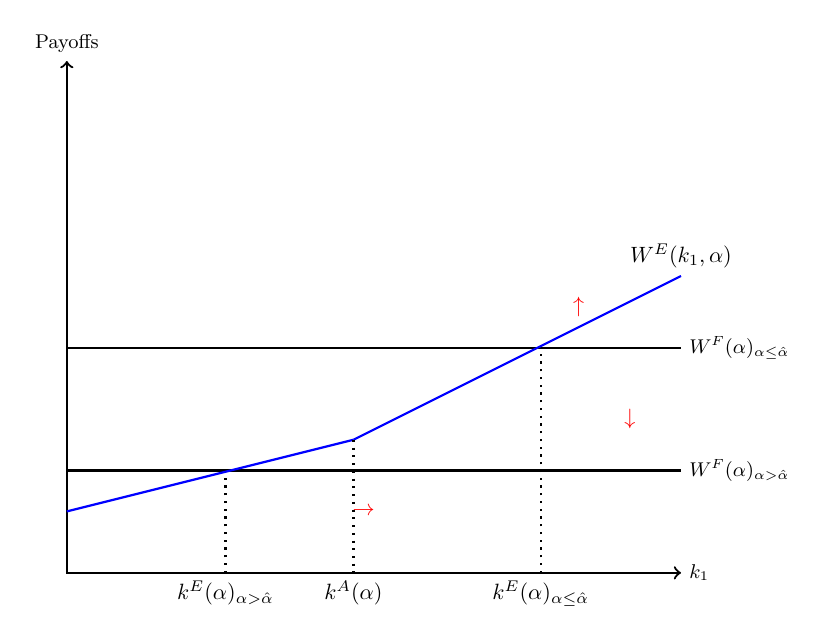
\begin{tikzpicture}[thick,scale=1.3, every node/.style={scale=0.8}]
\draw [<->] (0,5)node[above]{\small Payoffs} --  (0,0) -- (6,0);
\node [above] at (6,0) [right]{\small $k_1$};
%\draw[dotted] (0,1)--(6,4);
%\draw[dotted] (0,2)--(6,3.5);
 % node[midway, sloped, above] {task $A$ in firms}
\draw[] (0,1)--(6,1) node[right] {\small $W^F(\alpha)_{\alpha > \hat \alpha}$};
%node[midway, sloped, above] {task $B$ in firms}
\draw[] (0,2.2)--(6,2.2) node[right] {\small $W^F(\alpha)_{\alpha \leq \hat \alpha}$};

\draw[dotted](1.55,0)node[below]{$k^E (\alpha)_{\alpha >\hat \alpha}$}--(1.55,1);

\draw[dotted](4.63,0)node[below]{$k^E (\alpha)_{\alpha \leq \hat \alpha}$}--(4.63,2.2);

%\draw[dotted] (0,.5)--(6,3.5);
%\draw[dotted] (0,1)--(6,2.5);
 %node[midway, sloped, above] {task $A$ as entrepreneur}
\draw[blue] (0,.6)--(2.8,1.3);
% node[midway, sloped, above] {task $B$ as entrepreneur}
\draw[blue] (2.8,1.3)--(6,2.9)  ;
\node at (5,2.6) {\textcolor{red}{$\uparrow$}};

\node at (5.5,1.5) {\textcolor{red}{$\downarrow$}};
\node[above] at (6,2.9) {$W^E(k_1,\alpha)$};
\draw[dotted] (2.8,1.3)--(2.8,0)node[below] {$k^A(\alpha)$};
\draw[red] (2.9,0.6) node[]{$\rightarrow$};


\end{tikzpicture}



\caption{\footnotesize Lifetime utility of being an entrepreneur in period 1 ($W^E(k_1,\alpha)$) and lifetime utility of working for a firm in period 1 ($W^F(\alpha)$) as a function of  $k_1$. The arrows show how those values change as $\alpha$ increase: $W^F(\alpha)$ jumps downward as $\alpha$ increases from below to above $\hat \alpha$, while  $W^E(k_1,\alpha)$ and $k^A(\alpha)$ increase continuously with $\alpha$. } 
\label{fig:effect-labor}
\end{figure}


 The probability of becoming an entrepreneur in period 1 is therefore
 \[
 P^E_1(\alpha) = (1-\alpha) + \alpha \cdot \mbox{pr}\{k_1 \geq k^E (\alpha) \}.
 \]
 Note that the first part of the above expression is decreasing in $\alpha$, while the second one is increasing in $\alpha$, discontinuously so at $\alpha=\hat \alpha$.
 
It follows that, whenever $\hat \alpha > 0$ there is a non-monotonic relationship between labor market frictions and the probability of becoming an entrepreneur in period 1. %, due to the fact that as $\alpha$ increases, there are fewer necessity entrepreneurs but more learning and opportunity entrepreneurs: 
At $\alpha=0$ all agents are entrepreneurs, so the first order effect of an increase in $\alpha$ is a decrease in the number of entrepreneurs.  Instead, when $\alpha$ crosses $\hat \alpha$, contractual frictions makes it impossible to implement the efficient task allocation within firms, leading to a jump in the number of entrepreneurs.\footnote{The fact that the probability of becoming an entrepreneur is discontinuous is an artifact of the fact that firms success has constant value equal to 1. In a previous version of this paper, the value of firms' success was drawn randomly at the beginning of each period. In that version of the model, the probability of becoming an entrepreneur is continuous. Also in that version of the model, as $\alpha$ increases the probability of an efficient allocation within firms decreases. Hence, all results are identical to those presented here, but their derivation is significantly lengthier. }  Hence, it is possible that as the labor market becomes more efficient, fewer people become workers, preferring entrepreneurship instead.  

The following lemma summarizes these observations (its proof is omitted).
\begin{lemma}\label{lem: p1}
Whenever $\hat \alpha > 0$, there are $\alpha'<\alpha''<\alpha'''$ such that $P^E_1(\alpha')>P^E_1(\alpha'')$ and $P^E_1(\alpha'')<P^E_1(\alpha''')$.
\end{lemma}
\noindent Figure \ref{fig:parameter restriction} plots the parameter values for which Assumptions \ref{ass:sigma1}, assumption \ref{ass: necessary for learning}  and $\hat \alpha > 0$ hold, and the above lemma has bite. 



\begin{figure}
\centering 
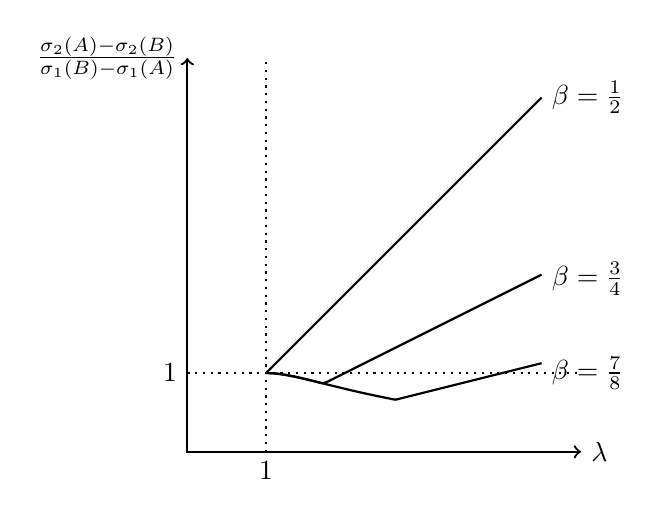
\begin{tikzpicture}[thick,scale=1, every node/.style={scale=1}]
\draw[<->](5,0)node[right]{$\lambda$}--(0,0)--(0,5)node[left]{$\frac{ \sigma_2(A)- \sigma_2(B)}{ \sigma_1(B)- \sigma_1(A)}$};
\draw[dotted](0,1)node[left]{$1$}--(5,1);
\draw[dotted](1,0)node[below]{$1$}--(1,5);
\draw[ domain=1:4.5, smooth, samples=50] plot (\x,{2*\x*max(1/2,1/(\x*\x+1))});
\node[right] at (4.5,4.5) {$\beta=\frac{1}{2}$};
\draw[ domain=1:4.5, smooth, samples=50] plot (\x,{2*\x*max(1/4,1/(\x*\x+1))});
\node[right] at (4.5,2.2) {$\beta=\frac{3}{4}$};
\draw[ domain=1:4.5, smooth, samples=50] plot (\x,{2*\x*max(1/8,1/(\x*\x+1))});
\node[right] at (4.5,1) {$\beta=\frac{7}{8}$};
\end{tikzpicture}
\caption{For different values of $\beta$, all values strictly above the curve satisfy Assumptions \ref{ass:sigma1}, Assumption \ref{ass: necessary for learning}  and $\hat \alpha > 0$. \label{fig:parameter restriction}}
\end{figure}

\begin{figure}
\setlength{\unitlength}{5cm}
\begin{picture}(2,1.5)
\put(0.15,0){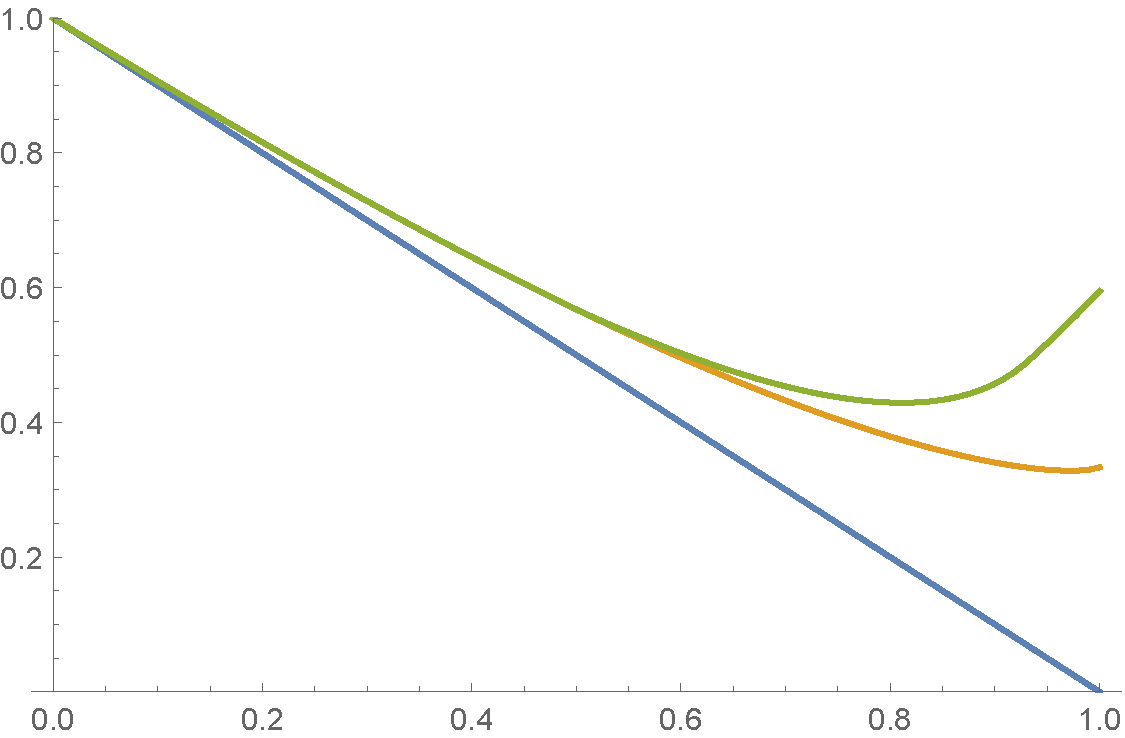
\includegraphics[scale=0.6]{P1}}
\put(1.9,.46){necessity + opportunity}
\put(1.75,.24){necessity}
\put(2.45,0.07){$\alpha$}
\put(1.5,.94){necessity + opportunity + learning}
\put(2.45,0.07){$\alpha$}
\begin{turn}{90}
\put(0.23,2.2){probability of entrepreneurship}
\end{turn}
\end{picture}
\caption{CHANGE THE FIGURE Motives for Entrepreneurship as a function of $\alpha$ 
($\beta=0.9$, $\lambda=1.5$, $p=0.45$, $h_A=0.9$, $l_A=0.1$, $h_B=0.4$, $l_B=0.6$)
}
\label{fig:P1}
\end{figure}

In period 2, instead, all those with $k_2>1$ become entrepreneurs. Those with  $k_2<1$ will be workers if they receive a wage offer, or if they were previously employed (in which case they can continue working for their former employer). Former entrepreneurs with $k_2<1$ who do not receive  a wage offer will remain entrepreneurs.  The probability of becoming an entrepreneur in period 2 is therefore:
\begin{align*}
%P_2^E(\alpha)&\equiv (1-\alpha)P_1^E(\alpha)+(1-(1-\alpha)P_1^E(\alpha))\mbox{pr}\{k_2>1\}\\
P_2^E(\alpha)&\equiv \mbox{pr}\{k_2>1\} + (1-\mbox{pr}\{k_2>1\}) (1-\alpha)P_1^E(\alpha) \\
&=\left(1-\frac{1}{\lambda}\right) +(1-\alpha )P_1^E(\alpha)\frac{1}{\lambda}.
\end{align*}

Having derived $P_1^E(\alpha)$ and $P_2^E(\alpha)$, we can now compute two commonly used measures of aggregate entrepreneurial activity: the probability of being a serial entrepreneur and the average probability of becoming an entrepreneur across periods.\footnote{In an overlapping generation extension of the model, $P_{(1/2)}$ is the probability that, at any given moment in time an agent is an entrepreneur.}
The probability of being a serial entrepreneur (that is, an entrepreneur in both periods) is
$$
P_{\mbox{serial}}^E(\alpha)\equiv P_1^E(\alpha) \cdot (1-\alpha +  \alpha \cdot \mbox{pr}\{k_2>1\})= P_1^E (\alpha)  \cdot \left(1-\frac{\alpha}{\lambda} \right),
$$
and the average probability of becoming an entrepreneur across periods:
\begin{align*}
P_{(1/2)}^E(\alpha)&\equiv \frac{1}{2} \left( P_1^E(\alpha) + P_2^E(\alpha) \right)\\
&= \frac{1}{2} \left( P_1^E(\alpha) \left(1+\frac{1-\alpha}{\lambda}\right) + 1 -\frac{1}{\lambda}  \right). 
\end{align*} 

Note that, like $ P_1^E(\alpha)$, both $P_{(1/2)}^E(\alpha)$ and $P_{\mbox{serial}}^E(\alpha)$ reach their maximum at $\alpha=0$ and are therefore decreasing for $\alpha$ sufficiently low. Furthermore, they both inherit $ P_1^E(\alpha)$ upward jump. These two observations imply the following corollary.


\begin{cor}\label{prop:probability-of-entrepreneurship}
Whenever $\hat \alpha > 0$, there are $\alpha'<\alpha''<\alpha'''$ such that
\begin{itemize}
    \item $P^E_{(1/2)}(\alpha')>P^E_{(1/2)}(\alpha'')$ and $P^E_{(1/2)}(\alpha'')<P^E_{(1/2)}(\alpha''')$, and
    \item $P^E_{\mbox{serial}}(\alpha')>P^E_{\mbox{serial}}(\alpha'')$ and $P^E_{\mbox{serial}}(\alpha'')<P^E_{\mbox{serial}}(\alpha''')$.
\end{itemize}


\end{cor}



Using the same parameter values as in Figure \ref{fig:P1}, a simulation shows indeed a non-monotonic relationship between $\alpha$ and these two aggregate measures of entrepreneurship (see Figure \ref{fig:Paverage}).



\begin{figure}[ht]
\setlength{\unitlength}{5cm}
\begin{picture}(2,1.5)
\put(0.15,0){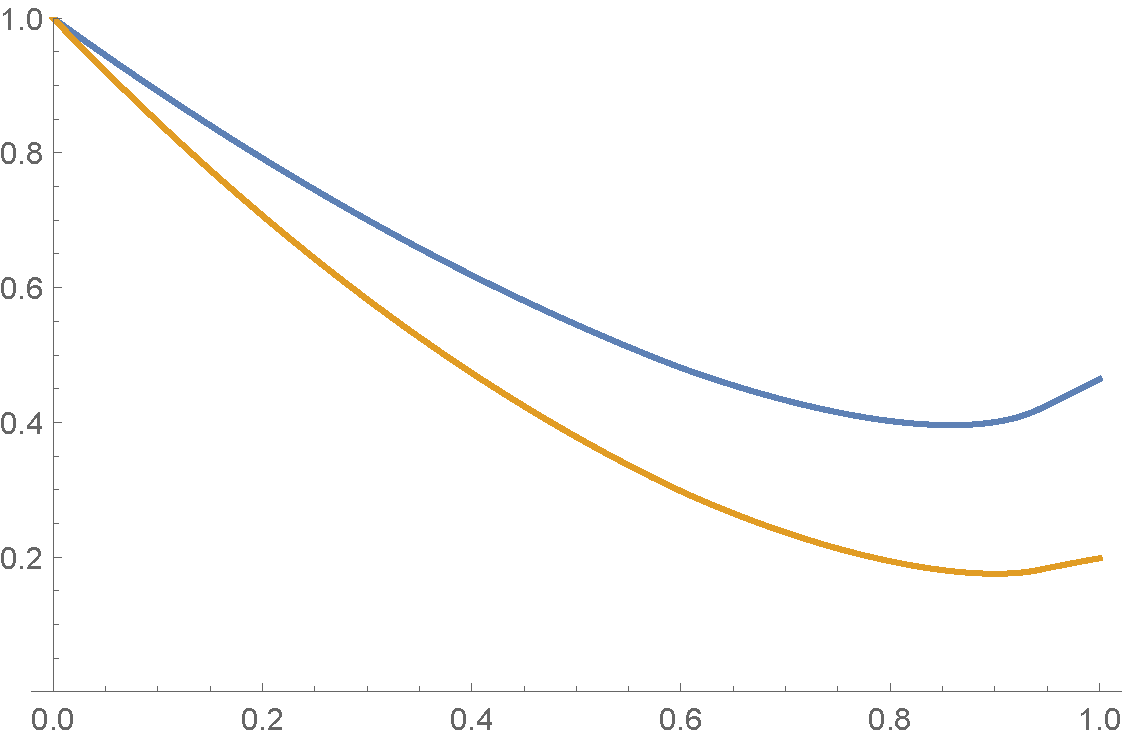
\includegraphics[scale=0.6]{Paverage}}
\put(1.85,.72){$P_{(1/2)}^E(\alpha)$}
\put(1.85,.24){$P_{\mbox{serial}}^E (\alpha)$}
\put(2.45,0.07){$\alpha$}
\begin{turn}{90}
\put(0.23,2.2){probability of entrepreneurship}
\end{turn}
\end{picture}
\caption{CHANGE Serial and Time Average Probabilities of Entrepreneurship as a function of $\alpha$.
($\beta=0.9$, $\lambda=1.5$, $p=0.45$, $h_A=0.9$, $l_A=0.1$, $h_B=0.4$, $l_B=0.6$)}
\label{fig:Paverage}

\end{figure}




\subsection{Types of entrepreneurs}

Labor market frictions affect not only the probability of becoming an entrepreneur, but also the type of projects pursued by entrepreneurs and their task allocation. Our framework allows us to distinguish between three types of entrepreneurship: 
\begin{itemize}
\item \textit{Necessity entrepreneurs}: are those who would prefer to work for a firm, but become entrepreneurs because they do not receive any wage offer. In period 1, they are a fraction $1-\alpha$ of the entrepreneurs with $k_1 < k^E(\alpha)$; in period 2, they are a fraction $1-\alpha$ of the entrepreneurs with $k_1 < 1$.
    \item \textit{Learning entrepreneurs}: are those who choose to become entrepreneurs and choose task $A$, when this is not possible within firms. That is, they are the period-1 entrepreneurs with project $k_1 \in [k^E(\alpha), k^A(\alpha)]$ for $\alpha > \hat \alpha$. Note that in period 2, independently of his profession, an agent is always allocated to the task that maximizes the period-2 probability of success. It follows that there are no learning entrepreneurs in period 2.
     \item \textit{Opportunity entrepreneurs}: are those who become entrepreneurs but are not motivated by learning, either because they could learn within firms or because they work on task $B$ as entrepreneurs. In period 1, learning entrepreneurs are those who choose entrepreneurship despite when task allocation in firms is efficient (i.e. those with $k_1 \geq k^E(\alpha)$ for $\alpha \leq \hat \alpha$) or who choose the same task allocation as in firms (i.e. those with $k_1 \geq \max\left\lbrace k^E(\alpha), k^A(\alpha) \right\rbrace$ for $\alpha > \hat \alpha$). Because task allocation within firms in period 2 is efficient, all old agents with $k_2 > 1$ are opportunity entrepreneurs.
\end{itemize}
Hence, in period 1 there can be necessity, learning or opportunity entrepreneurs, while in period 2 there can only be necessity or opportunity entrepreneurs.

Figure \ref{fig:types_of_entrepreneurship} shows how, in period 1, the proportion of different types of entrepreneurs changes with $\alpha$. Note that, by definition, learning entrepreneurs do not exist when the task allocation within firms is efficient, that is when $\alpha<\hat \alpha$. However, they always exist when $\alpha$ is sufficiently high.  For $\alpha=1$, the task allocation within firms is inefficient. Furthermore, by Assumption \ref{ass: necessary for learning}, $k^A(1)<1$, that is, an entrepreneur with project value equal to that of firms will choose task $A$. It follows that an agent with project value equal to that of firms becomes a learning entrepreneur: he chooses entrepreneurship over wage work, and work on task $A$ which is not possible in firms.  By continuity, there is a positive probability of becoming a learning entrepreneur for $\alpha$ sufficiently close to 1. The following Lemma summarizes these observations (its proof is omitted)
\begin{lemma}
Suppose $\hat \alpha>0$. Learning entrepreneurs exist for $\alpha$ sufficiently high but not for $\alpha $ sufficiently low.
\end{lemma}


\begin{figure}
    \centering
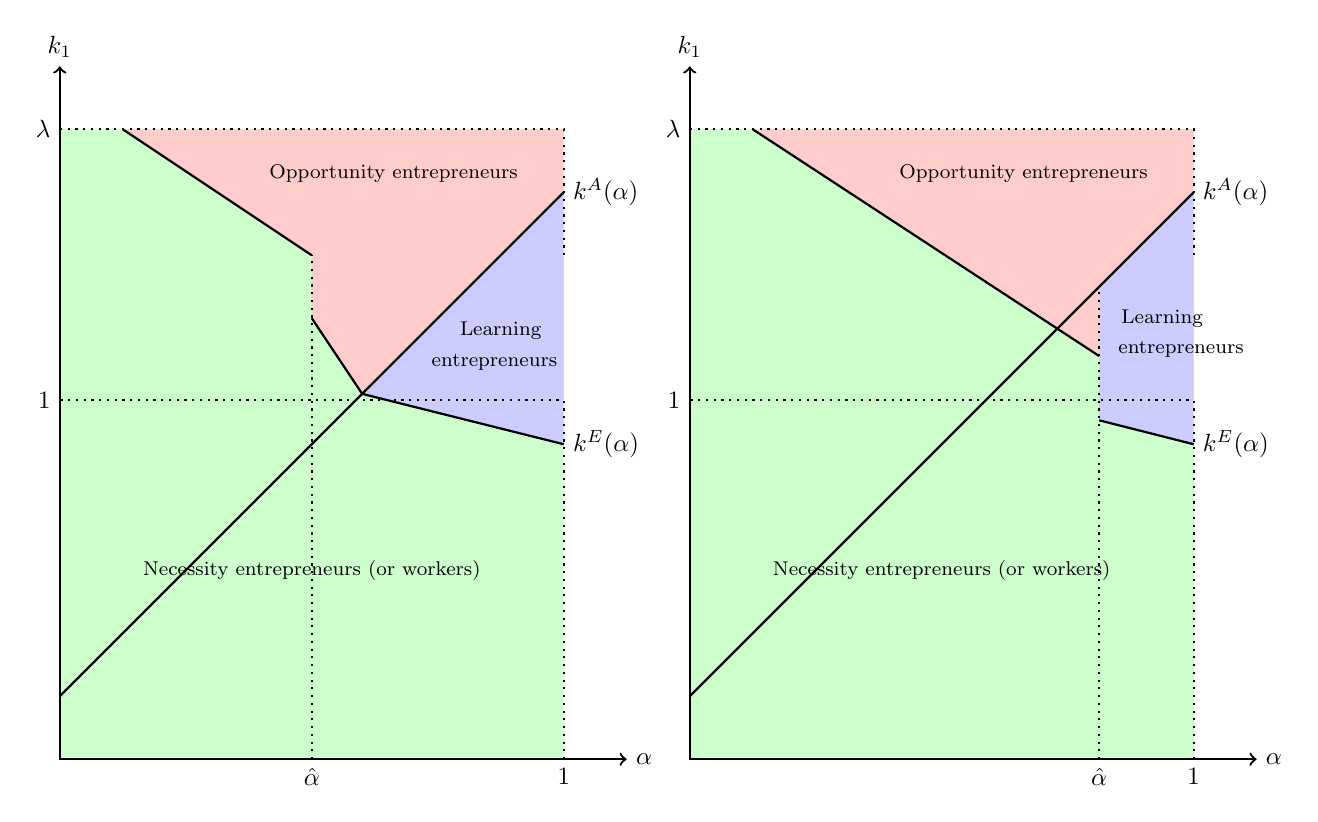
\begin{tikzpicture}[thick,scale=0.8, every node/.style={scale=0.9}]
\fill[green!20!white](0,0)--(0,10)--(8,10)--(8,0)--cycle;
\fill[blue!20!white](8,9)--(4.8,5.8)--(8,5)--cycle;
\fill[red!20!white](8,9)--(4.8,5.8)--(4,7)--(4,6)--(4,8)--(1,10)--(8,10)--cycle;
%\fill[green!20!white](8,5)--(4,6)--(4,8)--(4.8,5.8)--(1,10)--(0,10)--(0,0)--(8,0)--cycle;
\draw[<->](9,0)node[right]{$\alpha$}--(0,0)--(0,11)node[above]{$k_1$};
\draw[dotted](8,0)node[below]{$1$}--(8,5.7)--(0,5.7)node[left]{$1$};
\draw[dotted](8,8)--(8,10)--(0,10)node[left]{$\lambda$};
\draw(8,5)node[right]{$k^E(\alpha)$}--(4.8,5.8);
\draw(4.8,5.8)--(4,7);
\draw[dotted](4,0)node[below]{$\hat \alpha$}--(4,8);
\draw(4,8)--(1,10);
\draw(0,1)--(8,9)node[right]{$k^A(\alpha)$};
\node at (4,3) {\footnotesize Necessity entrepreneurs (or workers)};
\node at (5.3,9.3) {\footnotesize Opportunity entrepreneurs};
\node at (7,6.8) {\footnotesize Learning};
\node at (6.9,6.3) {\footnotesize entrepreneurs};
\begin{scope}[shift={(10,0)}]
\fill[green!20!white](0,0)--(0,10)--(8,10)--(8,0)--cycle;
\fill[blue!20!white](8,5)--(6.5,5.38)--(6.5,7.52)--(8,9)--cycle;
\fill[red!20!white](1,10)--(6.5,6.4)--(6.5,7.52)--(8,9)--(8,10)--cycle;
%\fill[green!20!white](8,5)--(4,6)--(4,8)--(4.8,5.8)--(1,10)--(0,10)--(0,0)--(8,0)--cycle;
\draw[<->](9,0)node[right]{$\alpha$}--(0,0)--(0,11)node[above]{$k_1$};
\draw[dotted](8,0)node[below]{$1$}--(8,5.7)--(0,5.7)node[left]{$1$};
\draw[dotted](8,8)--(8,10)--(0,10)node[left]{$\lambda$};
\draw(8,5)node[right]{$k^E(\alpha)$}--(6.5,5.38);%--(4.8,5.8);
%\draw(4.8,5.8)--(4,7);
\draw[dotted](6.5,0)node[below]{$\hat \alpha$}--(6.5,7.52);
\draw(1,10)--(6.5,6.4);
\draw(0,1)--(8,9)node[right]{$k^A(\alpha)$};
\node at (4,3) {\footnotesize Necessity entrepreneurs (or workers)};
\node at (5.3,9.3) {\footnotesize Opportunity entrepreneurs};
\node at (7.5,7) {\footnotesize Learning};
\node at (7.8,6.5) {\footnotesize entrepreneurs};

\end{scope}



\end{tikzpicture}
    \caption{Types of entrepreneurs in period 1. Left panel, low $\beta$ (and hence low $\hat \alpha$); right panel high $\beta$ (and hence high $\hat \alpha$) (note: the axes are not at scale).}
    \label{fig:types_of_entrepreneurship}
\end{figure}


A final observation is that opportunity entrepreneurs may work on task $A$ when also workers work on task $A$. This can happen in the right panel of Figure \ref{fig:types_of_entrepreneurship} (for $\alpha$ just above $\hat \alpha$ and project values between $k^E(\alpha)$ and $k^A(\alpha)$) but not on its left panel. However, the probability that entrepreneurs (independently on their type) work on task $A$ decrease as labor market frictions increase (i.e., $\alpha$ decrease). This is because as $\alpha$ decreases, $k^E(\alpha)$ increases, and hence entrepreneurs work on projects of higher value on average. At the same time, $k^A(\alpha)$ decreases, so that learning becomes less valuable for entrepreneurs. We summarize these observations in the following remark.

\begin{remark}
The fraction of entrepreneurs choosing $\tau_1=A$ strictly increases with $\alpha$
\end{remark}



\section{Additional Implications}\label{sec:implications}

\subsection{Wages of Past Workers and Past Entrepreneurs}\label{sec:wages of past workers vs entrepreneurs}

As already discussed in the literature review, our model generates novel predictions with respect to the wage of former workers relative to the wage of former entrepreneurs who change occupation.  As we established in section \ref{sec:equilibrium}, as $\alpha$ changes, the task allocations of workers and of entrepreneurs change in opposite directions. As $\alpha$ increases, workers are more likely to be allocated to task $\tau=B$ while entrepreneurs are more likely to choose task $\tau=A$.  More precisely, for $\alpha>\hat \alpha$ sufficiently large,  all workers are allocated to $\tau=B$ and a positive mass of entrepreneurs (the learning entrepreneurs) chooses instead task $A$. It follows, therefore, that for $\alpha$ sufficiently large the period 2 wage of a former entrepreneur is greater than the period-2 wage of a former worker. On the other hand, when $\alpha\leq \hat \alpha$ all workers are allocated to $\tau_1=A$, while entrepreneurs with a sufficiently valuable project will choose $\tau_1=B$. 

This difference in task allocation translate in differences in period-2 wage. This is immediate for workers who receive a wage offer and entrepreneurs, for which their period-2 wage equal their period-2 output within a firm. That is to say: if $\alpha>\hat \alpha$ the period-2 wage of former workers who receive a wage offer is lower than that of entrepreneurs who are hired by firms, while if $\alpha\leq \hat \alpha$ the opposite holds. However, the average wage of former workers also depends on the payoff of former workers who did not receive an outside offer. These workers will be paid less than the period-2 output generated within firms. However, by definition of $\hat \alpha$,   if $\beta$ is large (i.e. degree of contract incompleteness is low), $\hat \alpha$ is also large, so that even a small degree of labor market frictions can induce an efficient task allocation within firms. In this case, there exist values of $\alpha$ such that workers are more likely than entrepreneurs to work on task $A$, and at the same time the fraction of period-1 workers who do not receive a wage offer is low. For those values of $\alpha$, on average, former entrepreneurs  receive \textit{lower} wages compared to former workers of equivalent characteristics.
% 

There are unfortunately few empirical analysis relative to the compensations of former entrepreneurs who change occupation.  Nevertheless, our results are consistent with the existing empirical evidence. \citet{hamilton2000does} shows that US entrepreneurs who leave entrepreneurship and re-enter the labor market after some years earn higher wages than comparable workers: the median entrepreneur returning to paid employment after 10 years as an entrepreneur earns a wage that is 15\% higher than a comparable worker who never left employment.\footnote{%
See Table 6 and the discussion on pages 625-626 of \cite{hamilton2000does}. Hamilton notes that this result is consistent with the findings of \cite{evans1990}.  Both  \cite{daly2015long} and \cite{Hincapie2020} find similar results, using again US data.} See also \cite{luzzi2016individual}, who show that in Norway former entrepreneurs earn a positive wage premium.  Our model suggests an opposite result for high labor market friction economies (the wage of former entrepreneurs is lower than the wage of workers who have never left employment) which is consistent with the finding in \citet*{baptista2012former} for Portugal.\footnote{Neither \citet{hamilton2000does} nor \citet*{baptista2012former} discuss why an agent will leave entrepreneurship.}

%With respect to the instantaneous payoffs of workers relative to that of entrepreneurs, which one should be larger is ambiguous and depends on the model's parameters. For example, if $\lambda=\alpha=1$, there are only learning entrepreneurs who are more likely to fail and work on projects of lower values of firms. Hence entrepreneurs earn less than workers. But for other parameter values the result may change. For example, if $\lambda$  is sufficiently large, then entrepreneurs, on average, work on very valuable projects and therefore may earn more than workers.

\subsection{The Value of Entrepreneurial Failures}
A failure can be beneficial to an agent if it allows a better allocation of talent in the next period. As we will show shortly, failures have this property only if the agent has worked on the advanced task  \textit{and if} talent is horizontal. 

 Figure \ref{fig: success 2} illustrates how the maximum probability of success $\pi^M(p_t)$  varies as a function of the belief that the agent is a high type.\footnote{This probability is obtained by allocating an agent to the task with the highest probability of success, see Equation \ref{maxp} for the formal definition.} As is apparent,  when talent is vertical, the success probability is monotonically increasing, but if instead talent is horizontal, the success probability is non monotonic. That is, if talent is horizontal, an agent is least productive when there is probability $q^*$ that he is a high type, and productivity increases as the agent becomes more likely to be either a $h$ type or a $l$ type. 





\begin{figure}[h!]
    \centering
    \subfloat[Vertical case: $h_B>l_B$]{%
 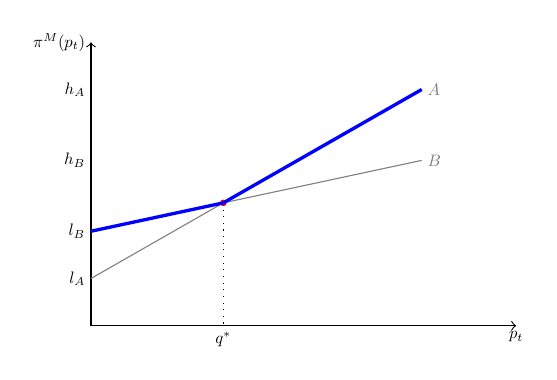
\begin{tikzpicture}[scale=0.6,transform shape]
\draw[->] (0,0) -- (9,0)node[below]{$p_t$};
\draw [->](0,0)--(0,6) node[left]{$\pi^M(p_t)$};
%%%%

\draw (0,5)  node[left]{$h_A$};
\draw (0,3.5) node[left]{$h_B$};
\draw (0,2) coordinate (B) node[left]{$l_B$};
\draw (0,1) coordinate (A) node[left]{$l_A$};
%
\draw[gray] (A)--(7,5) coordinate (C) node[right]{$A$};
\draw [gray] (B)--(7,3.5) coordinate (D) node[right]{$B$};
%Find intersection
 \fill[red] (intersection cs:
    first line={(A)--(C)},
    second line={(B)--(D)}) coordinate (I) circle (2pt);
%%%Projection
\draw[dotted] (I)--($(0,0)!(I)!(5,0)$) node[below]{$q^*$};
\draw[very thick,blue] (B)--(I)--(C);
\end{tikzpicture}}
%%%%%%%%%%%%%%%%%%%%%%%%%%%%%%%%%%%%%%%%%%%%%%%%%%%%%%%%%%%%%%%
    \centering
    \subfloat[Horizontal case: $h_B<l_B$]{%
 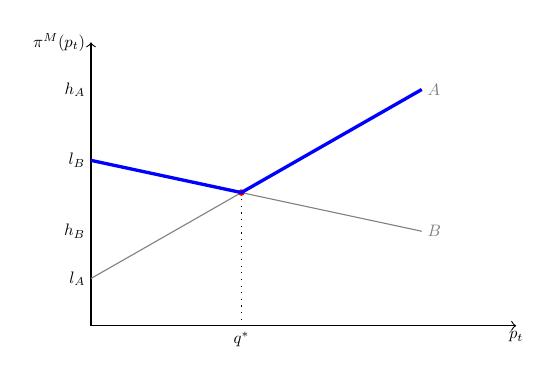
\begin{tikzpicture}[scale=0.6,transform shape]
\draw[->] (0,0) -- (9,0)node[below]{$p_t$};
\draw [->](0,0)--(0,6) node[left]{$\pi^M(p_t)$};
%%%%
\draw (0,5)  node[left]{$h_A$};
\draw (0,3.5) coordinate (B) node[left]{$l_B$};
\draw (0,2)  node[left]{$h_B$};
\draw (0,1) coordinate (A) node[left]{$l_A$};
%
\draw[gray] (A)--(7,5) coordinate (C) node[right]{$A$};
\draw [gray] (B)--(7,2) coordinate (D)node[right]{$B$};
%Find intersection
 \fill[red] (intersection cs:
    first line={(A)--(C)},
    second line={(B)--(D)}) coordinate (I) circle (2pt);
%%%Projection
\draw[dotted] (I)--($(0,0)!(I)!(5,0)$) node[below]{$q^*$};
\draw[very thick,blue] (B)--(I)--(C);
\end{tikzpicture}}
%%%%%%%%%%%%%%%
  \caption{Maximum probability of success as a function of belief $p_t$.}
  \label{fig: success 2}
\end{figure}
%
Remember from Section \ref{sec:learning} that when talent is vertical, failures reduce the probability of being a $h$ type (more so when the failure is at task $A$) since $h$ types are more likely to succeed than $l$ types at any task. Hence, when talent is vertical failures are always \textit{bad news} because they decrease the probability of success in period 2 relative to the initial probability of success, that is:
\[
\pi^M(p_2(\tau_1,0))<\pi^M(p_1) \mbox{ for all } \tau_1\in \{A,B\}.
\]
In the horizontal talent case, instead, failures at task $A$ increase the probability that the agent is a low type. By Assumption \ref{ass:sigma1}, such failures are \textit{good news } because they lead to an increase of the future probability of success (relative to no history). Instead, failures at task $B$ increase the probability that the agent is of type $h$, and may be good or bad news depending on the prior belief $p_1$: if $p_1$ is sufficiently close to $q^*$ failures at task $B$ are also good news; if instead $p_1$ is sufficiently low (for example, $p_1$ such that $\pi^M(p_2(B,0))<q$), then failures at task $B$ are bad news. The following Lemma formalizes these observations.
%
\begin{lemma}\label{lem: learning value of failures}
\begin{enumerate}[(i)]\setlength\itemsep{0em}
\item In the vertical-talent case failures are always bad news, that is,  $\pi^M(p_2(\tau_1,0))<\pi^M(p_1)$ for all $\tau_1\in \{A,B\}$.
\item In the horizontal-talent case, failures at task $A$ are always good news, that is, $\pi^M(p_2(A,0))>\pi^M(p_1)$. There is a threshold $q_B$ such that failures at task $B$ are bad news for $p_1<q_B$ and good news for $p_1>q_B$.
\end{enumerate}
\end{lemma}
%
Hence, the vertical view of talent implies that failures should reduce the probability of a future success. Instead, when talent is horizontal, failures can be ``good news'' depending on the task allocation. In this case, if labor market frictions are low (i.e., high $\alpha$) and the majority of entrepreneurs are learning entrepreneurs (i.e., $\lambda$ low), entrepreneurs will choose $\tau_1=A$ and a failure at this task leads to an increase in the future probability of success. This motivates the following proposition that relates the degree of labor market friction to the value of failures.
%
\begin{prop}
	\label{prop:probability-of-success} For a serial entrepreneur, the probability of succeeding as an entrepreneur in period 2 is increasing in $\alpha$. Furthermore
 \begin{enumerate}[(i)]\setlength\itemsep{0em}
\item If talent is vertical, failures are always ``bad news''. That is, the probability of succeeding in period 2 as an entrepreneur following an entrepreneurial failure in period 1 is below the initial probability of success $\sigma_1 (B)$ for all $\alpha$. 
\item If talent is horizontal, there exist parameter values such that failures are good news for $\alpha$ sufficiently high, and bad news for $\alpha$ sufficiently low.
\end{enumerate}
\end{prop}
%
The proposition is based on the fact that the degree of labor market frictions determine the task allocation chosen in period 1 by failed entrepreneurs: if $\alpha$ is large, failures are more likely to be generated by working on task $A$, while if $\alpha$ is low, they are more likely to be generated on task $B$. If talent is horizontal, a failure at task $A$ is a strong indication that the agent should instead work on task $B$ in the following period, while a failure at task $B$ increases the uncertainty relative to the optimal period-2 task allocation. It is possible that, in this case, failures are a good news for $\alpha$ large but bad news when $\alpha$ is low. If talent is vertical, instead, failures are always bad news, independently from the task. That is because low types are more likely to fail than high types at any task, meaning that a failure increases the probability that an agent is a low type and will fail in the future.


With respect to the existing evidence, in the US entrepreneurial failures seem to lead to entrepreneurial success. For example, \citet*{gompers2010performance} show that entrepreneurs who previously failed are marginally more likely to succeed than first time entrepreneurs.\footnote{See also \cite{NBERw20312}, who use data from Texas to show that the past experience as an entrepreneur predicts entrepreneurial success. This is consistent with our model for the case of ``low labor market frictions'' in which, in period-1, entrepreneurs are more likely to choose an informative task allocation than workers. It follows that, in period 2, an entrepreneur who was formerly an entrepreneur is more likely to succeed than an entrepreneur who was formerly a worker.}
 %This is, again, consistent with our model because when the task allocation of entrepreneurs favors learning, failures can be informative with respect to the future task allocation. 
Again the evidence available for Europe tells a very different story.  
Using German data, \citet*{gottshalkGreene2012} show that entrepreneurs who have previously failed are subsequently more likely to fail than first time entrepreneurs. %, which is consistent with our finding that for intermediate labor-market frictions there are no learning entrepreneurs in the model.
Our model explains these different values of failure if talent is \emph{horizontal}: different agents have  
an absolute advantage at different tasks.  Instead, when talent is \emph{vertical} (that is, the same agent has an absolute advantage at all tasks) failures are always bad news, independently of the level of labor market frictions, a finding which seems counterfactual. 

\subsection{Age Profile of Entrepreneurs}
At $\alpha=1$, there are no necessity entrepreneurs. Furthermore, in period 2, and agent with project value equal to that of firms is indifferent between joining a firm or becoming an entrepreneur. However, in period 1 such agent strictly prefers to become an entrepreneur, because this allows him to learn: to implement task $A$ instead of $B$. 
By continuity, therefore, for $\alpha$ sufficiently large young agents are more likely than old agents to become entrepreneurs.

%As $\alpha=1$ since there are no necessity entrepreneurs and learning entrepreneurs only in period 1, there are more young than old entrepreneurs. As $\alpha=0$, the necessity motive is first order and 

%\footnote{This is most evident for very low values of $\alpha$, because \[\frac{\partial P_2(\alpha)}{\partial \alpha}|_{\alpha=0}=\frac{1}{\lambda}\left(\frac{\partial P_1(\alpha)}{\partial \alpha}|_{\alpha=0} -1\right) <\frac{\partial P_1(\alpha)}{\partial \alpha}|_{\alpha=0} ,\] which implies that $P^E_1(\alpha)>P^E_2(\alpha)$ near $\alpha=0$. }
%
For lower values of $\alpha$, however,  other effects come into play. % Remember that workers can continue working for their previous employer. It follows that as age increases, an agent is more likely to receive a wage offer and to leave entrepreneurship.  By this logic, old people should be less likely to be entrepreneurs than young people.
For example, in period 1 agents anticipate that, if they become entrepreneurs, they may not be able to find a job in the future. This concern is absent in period 2. It is therefore possible that, for some intermediate $\alpha$, there are more entrepreneurs in period 2 than in period 1. 

We are not aware of any evidence linking  the probability of becoming an entrepreneur at different ages with the degree of labor market friction. Using US data, \cite{Hincapie2020} shows that people are the most likely to become entrepreneurs when in their mid thirties.  This is consistent with our model for the ``low labor market friction'' case provided that we interpret ``mid thirties'' as part of  period 1 of the model (which is the only period of our model in which learning is valuable).
A  recent  paper by \cite*{Azoulay2020} shows that old entrepreneurs are more likely \textit{to succeed} than young entrepreneurs. This is consistent with the model, because experience generates learning (independently from an agent occupation or task allocation), which can then be used in the choice of task allocation.

\subsection{Other comparative statics}

The degree of contracting frictions is measured by $\beta$, with higher values corresponding to lower frictions.  For given $\alpha$, as $\beta$ increases firms are better able to capture the value of learning their workers' talent. As a consequence, they are more likely to implement task $\tau_1=A$, thus eliminating the learning motive for entrepreneurship. Hence, for given $\alpha$, increasing $\beta$ (weakly) decreases the probability of becoming and entrepreneur.

Increases in $\lambda$ instead lead to an increase in the probability of becoming an entrepreneur. This is because of a direct effect: good ideas are more likely, leading to more opportunity entrepreneurship. Furthermore, \textit{future} good ideas are more likely which implies two things. First, workers who do not receive a wage offer at the beginning of period 2 are more likely to leave their firm, therefore making learning less likely to occur within firms (i.e., $\hat \alpha$ decreases). Second, learning becomes more valuable because future successes are more valuable. Overall, the proportion of learning entrepreneurs increases. 



\subsection{Output}\todo[inline]{maybe this should go in the "main" section (section 5). It is kind of neat and fits well next to the fact that entrepreneurship is non-monotonic in $\alpha$}
In period 1 a fraction $1-\alpha$ of the population will not receive a wage offer and is forced into entrepreneurship, while a fraction $\alpha$ of the population chooses entrepreneurship or wage work depending on the two period output generated by these two options. Hence, the two-period total expected output in the economy is
\[
(1-\alpha) \cdot E[W^E(k_1,\alpha)] + \alpha \cdot E[ \max\left\lbrace W^E(k_1,\alpha), W^F(\alpha) \right\rbrace ].
\]
Therefore, for a fixed $W^F(k_1,\alpha)$, total expected output increases with $\alpha$ both because fewer agents become necessity entrepreneurs, and because $E[W^E(k_1,\alpha)]$ increases with $\alpha$. At the same time, $W^F(\alpha)$ has a downward discontinuity at $\alpha=\hat \alpha$, and is constant otherwise.  Total output is therefore non-monotonic in $\alpha$: it is increasing for $\alpha \neq \hat \alpha$ but has downward discontinuity at $\alpha=\hat \alpha$.




\section{Conclusion}\label{conclusion}
%
We have shown that, when contracts are incomplete, occupational choice can be partially explained by the difference in decision rights across occupations. This approach allows us to highlight a novel motive for entrepreneurship (learning one's comparative advantage) that is especially important when firms compete fiercely for workers. The literature already showed  that learning one's comparative advantage is an important driver of \textit{career} choices and wage dynamics across firms. We highlight its importance in explaining \textit{occupational} choices and the resulting wage dynamics.

In order to focus on this motive for entrepreneurship, we have ignored other important determinants of entrepreneurial activity, such as financial constraints, learning by doing, or the possibility of working on multiple tasks. 

Financial constraints are a barrier to entry into entrepreneurship. In our model, when entrepreneurs face financial constraints, the effect of labor market frictions on entrepreneurial activity will in fact be stronger. Indeed, if the labor market is frictionless, firms' competition insures that workers are able to appropriate the full benefit of learning.  Hence firms adopt a less informative task allocation independently of the importance of financial constraints, and some agents may become learning entrepreneurs. On the other hand, when labor-market frictions are severe, financial constraints limit the exit of workers into entrepreneurship and therefore increase the ability of firms to appropriate the benefit of learning.\footnote{On the role of financial constraints, see \citet{Hellmann:2007tk}, who shows that cash constraints shape the way ideas are financed, within or outside the firm, and \citet{tervio_superstars_2009}, who argues that, absent long-term contracts, financial constrains may prevent optimal talent discovery in firms.}  The presence of financial constraints, therefore, increases the effect of a change in $\alpha$ on whether learning occurs within or outside firms.


%In this case, therefore, labor-market frictions and financial constraints are complementary since they both increase the likelihood that learning will occur within firms.
%However, if labor market frictions are sufficiently low, independently of the presence of financial constraints, learning cannot occur within firms and some agents may become learning entrepreneurs.

There is an element of learning by doing in our model because agents acquire information about their comparative advantage, are better able to match their talent to a task, and therefore increase their productivity over time.  We do not however allow agents to increase their productivity on a given task by simply working on that task, that is, there is no task-specific human capital accumulation (see \citealp{gibbons1999theory} and \citealp{gibbons2004task}).
Our results stand as long as this increase in productivity is small compared to the benefit of learning one's comparative advantage.  
  

We have assumed that the production process involves only one task. By contrast, \citet{lazear2004balanced} assumes that workers work at a single task while entrepreneurs work at multiple tasks. He shows, both theoretically and empirically, that people with a more balanced skill set enter entrepreneurship. \citet*{aastebro2011stars}, building on \citet{lazear2004balanced}, propose a model in which agents choose between self-employment (in which case they work on multiple tasks) and wage work (in which case they are allocate to a specific task). Exogenous frictions prevent both the efficient assignment of agents to firms, and also the efficient assignment of workers to tasks. These frictions are the reason why some agents may become self employed. Both in \citet{lazear2004balanced}  and \citet{aastebro2011stars} agents' productivity at different tasks are perfectly known, and hence there is no learning. This implies that, for example, these models do not  make predictions with respect to the wage of former entrepreneurs.
It would be interesting to add uncertainty about talent to Lazear's framework, and study whether learning affects agents' occupational choices. This extension is left for future work. 

Finally, one may be tempted to interpret the case of high labor market frictions as illustrative of developing countries, and there is indeed ample evidence that many people living in developing countries are ``reluctant'' entrepreneurs  \citep{pooreconomics}. However, we refrain from this temptation. We use the model to explore the effect of labor market frictions keeping everything else constant. This may be a reasonable way to proceed when comparing countries (such as the US and European countries) that have different levels of labor market frictions but are otherwise similar in their contracting abilities, the development of their financial markets, and their level of human capital. But this is hardly the case for developing countries.  These other dimensions are not part of our model but are likely to affect the type, frequency and market rewards of entrepreneurial ventures.



%{\color{red} The most relevant simplification we made is the assumption that the distribution of firms' and entrepreneurs' project value is constant. For example, in the model both old and young agents draw projects from the same distribution, but  old agents may have more experience and therefore may draw projects with higher expected value than young agents.}
%\todo[inline]{whether a young agent is more or less likely than an old agent to become an entrepreneur is not straightforward and depends on labor market frictions. If labor market frictions are high, there is no learning motive. At the same time, a young agent who becomes entrepreneur may not find a job tomorrow (which is not a concern for old agents). As a consequence, old agents are more likely than young agent to become entrepreneurs. On the other hand, if labor market is frictionless, then young agent are more likely than old agent to become entrepreneurs because of learning.  } {\color{red} For this reason, we are reluctant to use our model to make predictions relative to age-profile of entrepreneurs. Also, as already discussed, high labor-market frictions may create unfilled vacancies, distort technological choices, and therefore reduce the average project value of firms and entrepreneurs. However, it is unclear what the impact of labor market frictions on the firms' project distribution relative to that of entrepreneurs should be, and it is therefore unclear how labor market frictions should affect the relative productivity of firms and entrepreneurs.} 




\appendix
\section{Mathematical Appendix}\label{mathematical appendix}

% \subsection*{Proof of lemma \ref{lem:When-entrepreneurship}}

% The value of entrepreneurship is:
% \[
% \max\{V(\tau_1=1),V(\tau_1=0)\}
% \]
% Where 
% \[ V(\tau_1=1)	=	q p_0 \left(k_1+q\right)+(1-qp_0)\cdot q\cdot\mbox{max}\left\{ \frac{p_0(1-q)}{1-p_0q},\frac{1-p_0}{1-p_0q}\right\}, 
% \] 
% and \[
% V(\tau_1=0)	=	q(1-p_0)\left(k+q\right)+(1-q(1-p_0))\frac{qp_0}{1-q(1-p_0)}.
% \]
% are the values of working on task $1$ and $0$ respectively for a given entrepreneurial project $k_1$. The vale of working for a firm is
% \[
% V_w	=	q p_0 \left(K_1+q\right)+(1-qp_0)\cdot q\cdot\mbox{max}\left\{ \frac{p_0(1-q)}{1-p_0q},\frac{1-p_0}{1-p_0q}\right\}, 
% \]

% The lemma follows by solving for
% \[
% \max\{V(\tau_1=1),V(\tau_1=0)\}>V_w.
% \]

\subsection*{Conditions for $\sigma_2(A)>\sigma_2(B)$.}\label{sec:appendix-learning}

\begin{prop}\label{prop:nsc_learning}
In the vertical talent case $\sigma_2(A)>\sigma_2(B)$ if and only if 
\begin{equation}\label{eq: learning}
p_1>\left(1+\frac{h_A}{l_A}\frac{h_A-h_B}{l_B-l_A} \right)^{-1}.
\end{equation}
In the horizontal talent case  $\sigma_2(A)>\sigma_2(B)$ if condition \eqref{eq: learning} holds and
\begin{align*}
h_A-l_A>l_B \cdot h_A-l_A \cdot h_B >l_B-h_B.
\end{align*}
\end{prop}
\begin{proof}

%\paragraph{Necessary condition for informativeness.}  
Independently of the task assignment in the first period, Bayesian updating implies that 
\begin{equation}\label{mean}
\mathbb E_{s_1\in\{0,1\}}\pi (\tau_1,p_2(\tau_1,s_1)) p_2(\tau_1,s_1)=p_1.
\end{equation}
Because of Assumption \ref{ass:sigma1}, there is a realization of $s_1$ such that the posterior $p_2(\tau_1,s_1)$ is inferior to $q^*$, leading to  task $B$ being adopted in period 2. Since the expected probability of success $\pi^M(p_t)$ is linear when $p\leq q^*$, a necessary condition for $A$ to be more informative than $B$ is that $\max_{s_1}p_2(A,s_1)>q^*$.  Because in both the vertical and horizontal cases $\frac{h_A}{l_A}>\frac{1-h_A}{1-l_A}$, the maximum posterior following task $A$ is achieved following a success. More informativeness of $A$ therefore requires that $p_2(A,1)>q^*$, that is
\begin{equation}\label{q}
p_1 > q_A\equiv  \left(1+\frac{h_A}{l_A}\frac{h_A-h_B}{l_B-l_A}\right)^{-1}
\end{equation}
%
\paragraph{Sufficient condition for (weak) informativeness.} %Here we derive a sufficient condition for task $B$ \textit{not to be more informative} than task $A$; the combination of this condition together with the previous condition $p_1>q$ will then be sufficient for informativeness of $A$. 

Since the maximum probability of success is a convex function of the posterior, whenever the distribution of posteriors following $\tau_1=A$ is a mean preserving spread of the distribution of the distribution following $\tau_1=B$, we will have $\sigma_2(A)\geq \sigma_2(B)$. Using our previous remark that $\max_{s_1}p_2(A,s_1)=p_2(A,1)$, the distribution of posteriors following $A$ is a mean-preserving spread of the distribution following $B$ whenever:
\begin{align}\label{mps}
p_2(A,0) < &\min_{s_1}p_2(B,s_1)<p_1<\max_{s_1}p_2(B,s_1) < p_2(A,1). \tag{MPS}
\end{align}
Under the above condition, $\sigma_2(A) = \sigma_2(B)$ if and only if $p_1\leq q_A$, that is if and only if no matter the task allocation and the realization of success and failure in period 1 the agent is always allocated to task $B$ in period 2. Hence, \eqref{mps} and $p_1> q_A$ are sufficient for  $\sigma_2(A) > \sigma_2(B)$.

%
When talent is vertical, $h_A>h_B>l_B>l_A$, and
the posteriors are ordered as
\begin{equation*}
p_2(A,0)<p_2(B,0)<p_1<p_2(B,1)<p_2(A,1).
\end{equation*} 
and \eqref{mps} is automatically satisfied.

%
When talent is horizontal,  $l_B>h_B$ implies that 
\[  p_2(B,1)<p_1<p_2(B,0) \;\text{ and }\; p_2(A,0)<p_1<p_2(A,1), \]
but not necessarily \eqref{mps}. The distribution of posteriors following $A$ is a mean preserving spread of the distribution of posterior following $B$ whenever $p_2(A,1)>p_2(B,0)$ and $p_2(A,0)<p_2(B,1)$. Simple algebra shows that these conditions are equivalent to $h_A-l_A>l_Bh_A-l_Ah_B >l_B-h_B$, which is therefore sufficient for $\sigma_1(A)<\sigma_1(B)$ but $\sigma_2(A)>\sigma_2(B)$ in the horizontal case.
%

\end{proof}










\subsection*{Proof of Lemma \ref{lem: learning value of failures}}



When talent is vertical, we showed in the proof of Proposition \ref{prop:nsc_learning}  that $p_2(A,0)<p_2(B,0)<p_1$, which implies that failures always reduce the probability of being a $h$ type (more so when the failure is at task $A$). Because the function $\pi^M(p_t)$ is monotonically increasing, we have the inequalities $\pi^M(p_2(A,0))<\pi^M(p_2(B,0))<\pi^M(p_1)$, and hence and failures decrease the probability of success in period 2 relative to the initial probability of success.

 
Instead, in the horizontal case low types are more likely to succeed at task $B$ than high types and therefore $ p_2(A,0)<p_1<p_2(B,0)$. Furthermore, the function $\pi^M(p_2)$ is decreasing for $p_2<q^*$ and then increasing, implying that  $\pi^M(p_2(A,0))>\pi^M(p_1)$. Note also that there is a threshold value of $p_1$ below which $\pi^M(p_2(B,0))<\pi^M(p_1)$ (failures at $B$ are bad news) and above which  $\pi^M(p_2(B,0))>\pi^M(p_1)$ (failures at $B$ are good news). If $p_1$ is so low that  $p_1<p_2(B,0)<q^*$, then quite immediately failures are bad news. Whenever instead  $p_1<q^*<p_2(B,0)$ we have that $\pi^M(p_1)$ is monotonically decreasing in $p_1<q^*$, but $\pi^M(p_2(B,0))$ is monotonically increasing in $p_1$. The statement therefore follows by continuity.


\section*{Proof of Proposition \ref{prop:probability-of-success}}

 For given project value $k_1$ the probability that an entrepreneur sets $\tau_1=A$ increases with $\alpha$. At the same time $\alpha$ determines the set of $k_1$ that will be pursued by agents who receive a wage offer and become entrepreneurs.  For these agents, as $\alpha$ increases, the set of projects that are pursued enlarges: smaller $k_1$ are pursued by entrepreneurs. These projects are the ones for which the entrepreneurs are more likely to choose $\tau_1 =A$. Overall, the probability of setting $\tau_1=A$ increases with $\alpha$, which implies that the probability of succeeding in period 2, also increase with $\alpha$. 
 
 The second part of the Proposition follows by Lemma \ref{lem: learning value of failures}. In the vertical talent case the probability of period-2 success following a failure is always below the initial probability of success $\pi^M(p_1)\equiv\sigma_1(B)$. In the horizontal talent case failures at task $A$ are always good news, while if $p_1<q_B$ failures at task $B$ are bad news.  Hence, if talent is horizontal, $\alpha=1$ and $\lambda$ low, for any $p_1<q_B$  the majority of entrepreneurs are motivated by learning and set $\tau_1=A$. In this case, failures are good news. When  $\alpha \leq \hat \alpha$, entrepreneurs are either opportunity entrepreneurs or necessity entrepreneurs. They set $\tau_1=A$ whenever $k_{1}\leq k^A(\alpha) $, and $B$ otherwise. By definition of $k^A(\alpha)$, as $\alpha$ decreases, entrepreneurs are more likely to choose task $B$. Also, for given $\alpha$, in the limit case $p_1 \rightarrow 0$, we have $ \sigma_2(A) \rightarrow \sigma_2(B)$ and all entrepreneur choose task $B$ and entrepreneurial failures are bad news. By continuity, there exists a $p_1$ and $\alpha<1$ such that entrepreneurial failures are bad news.

% \section*{Renegotiation of Bonus Payment}\label{renegotiation}
% 
% We assumed in the body of the paper that firm and worker cannot renegotiate the contingent part of the wage $b$. For the case $\alpha=1$, this assumption implies $b\leq \underline \beta K_t$. Here allow the agents to avoid project termination by renegotiating the contingent part of the wage.
% 
% Assume $\alpha=1$. Whenever $b>\beta_{i,t}K_t$, by Nash bargaining project termination will be avoided and the worker will get a  renegotiated bonus of $\beta_{i,t}K_t/2$ (remember that $\beta_{i,t}$ is observable). Hence, whenever the parties agree on a $\underline \beta K_t<b<\overline \beta K_t$, the expected contingent part of the wage is:
% 
% \begin{align*}
% {b}(b,K_t,\underline \beta)=& \mbox{pr}\{\beta_{i,t} K_t \leq b\} \frac{K_t b}{2} + (1-\mbox{pr}\{\beta_{i,t} K_t \leq b\}) b\\
% =&\frac{b^2 - K_t b \underline \beta + 4b -2\underline \beta b -\frac{2b^2}{K_t}}{4(1-\underline \beta)}
% \end{align*}
% which is the realized payment in case of success, taking the expectation with respect to $\beta_{i,t}$. Note that ${b}(b)<b$ for $b>\underline \beta K_t$. However, it may be the case that ${b}(b)>\underline \beta K_t$ for some $b>\underline \beta K_t$. Hence, by allowing for renegotiation, the realized contingent part of the wage may pushed higher that without renegotiation. 
% 
% Define 
% $$
% b^\star(K_1,\underline \beta) =\mbox{argmax}_{b\in[\underline \beta K_1, (1-\underline \beta) K_1]}  \left\{ \frac{b^2 - K_1 b \underline \beta + 4b -2\underline \beta b -\frac{2b^2}{K_1}}{4(1-\underline \beta)} \right\} 
% $$
% so that $\min\{K_1,b^\star(K_1,\underline \beta) \}$ is highest bonus payment that can be offered. In case $\min\{K_1,b^\star(K_1,\underline \beta) \}<K_2$ lemma \ref{lem:short run-max-by-firms} holds also here: when deciding on task allocation, the firm prefers a success and therefore chooses $\tau_1=1$. However, in case $\min\{K_1,b^\star(K_1,\underline \beta) \}=K_2$ when deciding on task allocation the firm is indifferent between failure or success, and between $\tau_1=1$ or $\tau_1=0$. In this case, there is an equilibrium in which the firm allocates the worker to task $\tau_1=0$.
% 
% \begin{figure}   \centering
% \subfloat[$\underline{\beta}=0$]{\includegraphics[scale=0.34]{pasted1}} \\
% 
% \subfloat[$\underline{\beta}=.4$]{\includegraphics[scale=0.34]{pasted2} 
% }\\
% \subfloat[$\underline{\beta}=.7$]{\includegraphics[scale=0.34]{pasted3}
% }\\
% \subfloat[$\underline{\beta}=.9$]{\includegraphics[scale=0.34]{pasted4}
% }
% \caption{Maximum contingent payment implementable \label{fig:renegotiation}}
% 
% \end{figure}
% 
% We determine whether $\tau_1=0$ is implementable via numerical simulations, which we report in figure \ref{fig:renegotiation}. In each quadrant, it is possible to implement $\tau_1=0$ if and only if the line marked as $b^\star$ is above the 45 degrees lines. For values of $\underline \beta$ sufficiently low, the set of projects for which it is possible to implement $\tau_1=0$ is different from the set of project for which it is optimal to implement $\tau_1=0$. In particular, $\tau_1=0$ is implementable for high-value projects, but it is optimal for low value projects. Hence, for $\underline \beta \leq .7$, lemma \ref{lem:short run-max-by-firms} holds here as well, and some agents may become entrepreneurs to learn their type. On the other hand, when $\underline \beta \geq .9$, it is possible to implement $\tau_1=0$ within firms when this task allocation is optimal. Hence the learning motive for entrepreneurship disappears.
% 
% 






\section{Unobservable Task Allocation}\label{app:unobservable}

When past task allocation is not observable outside of the firm, at the beginning of period 2 there may be asymmetry of information between firms and any agent who did not work for the same firm previously. %From the point of view of a firm, after observing a success, the agent is either type $p=1$ or $p=0$. After observing a failure, an agent can be one of two types, corresponding to the beliefs obtained under each task allocation as in \eqref{learning}. 
%In this situation, there are several possible equilibria, because firms' period 2 beliefs and period 2 wages affect period 1 task allocation, and vice versa. We consider two classes of equilibria:  equilibria in which for every observable history, firms offer a menu of contracts (screening); and equilibria in which for every observable history, firms offer a single contract (no screening). 
We restrict our analysis of this problem to the case $\alpha=1$. Our goal is to show that the basic finding of the model in the text persists:  the learning motive for entrepreneurship emerges when $\alpha$ is high. (It is quite immediate to see that as $\alpha$ decreases the learning motive for entrepreneurship disappears.)

%Note that, whenever $\alpha=1$, the fact that project termination is unobservable is not relevant. Remember that project termination leads to a failure with probability 1. For any market belief regarding the worker's productivity in case of failures, the worker prefers not to terminate the project, and strictly so if $b>0$. Competition among firms assures that $b\leq \underline \beta K_1$. Hence, project termination never occurs in equilibrium: in case of failures, the only uncertainty is relative to period 1 task allocation.


\paragraph*{Screening equilibria.}

Suppose that in period 2, for every observable history,  firms offer a contract for every possible type, where a contract has the form $\{b,f,\tau_2\}$ i.e., a bonus, fixed payment, and a task allocation. Clearly, if the agent produced a success in the previous period, a menu of contracts $\{b,f,\tau_2=A\}$ and $\{b',f',\tau_2=B\}$ such that $f+qb=f'+qb'=1$ is an equilibrium screening menu of contracts, because each firm makes zero profits, agents of different types prefer different contracts (strictly so if $b,b'>0$), and the firm has no incentive to implement a task allocation that is different from that specified in the contract.\footnote{Note that this contract amounts to delegating task allocation to the worker. Delegation is possible because, in period 2, workers and firms have aligned preferences regarding task allocation.}

However, in order to use such contracts, it must be the case that conditional on a given outcome $s_1$, those who worked at different period-1 tasks maximize period-2 probability of success by working at different period-2 tasks. In other words, after observing a failure, screening is possible if those who worked at task $\tau_1=A$ should work in period 2 on task $\tau_2=B$, and vice versa. Similarly, after observing a success, screening is possible if those who worked at task $\tau_1=A$ should work in period 2 again on task $\tau_2=A$, and the same for those who worked on task $\tau_1=B$. 

This condition is never satisfied when talent is vertical. In this case, successes (whether at task $\tau_1=A$ or task $\tau_1=B$) increase the probability that the agent is of type $h$ and that he should be allocated to task $\tau_2=A$. Similarly failures (whether at task $\tau_1=A$ or task $\tau_1=B$) increase the probability that the agent is of type $l$ and that he should be allocated to task $B$. Hence, in general, screening is not possible when talent is vertical.\footnote{It may still, however, be possible to screen conditional on a given period-1 outcome, but not on the other outcome. }

Screening is possible whenever talent is horizontal and $p_1$ is sufficiently close to $p^\star$. In this case, successes at task $\tau_1=A$ or task $\tau_1=B$ make it more likely that the agent should work at that task in period 2 as well. Similarly, failures at task $\tau_1=A$ or task $\tau_1=B$ makes it more likely that the agent should work at the other task in period 2. If the initial prior is sufficiently uncertain, conditional on the outcome $s_1$ there is a one-to-one correspondence between $\tau_1$ and $\tau_2$ maximizing period-2 probability of success.





% those who worked at task $\tau_1=1$ maximize the probability of success in period 2 by working on a task that is fi

% If the agent produced a failure in period 1, then screening on the base of task allocation is possible only if agents who failed at task $\tau_1=1$ are the most productive at task 0 in period 2, i.e., if $p_0(2-q)<1$. If we write the bonus payment as a fraction $\eta$ of total output, and use the zero profit condition on each contract, incentive compatibility implies
% $$
% 1> \mu' (1- \frac{qp_0}{1-q(1-p_0)} ) +(1-\mu')\frac{q(1-p_0)}{1-p_0 q}
% $$
% $$
% 1> \mu (1- \frac{q(1-p_0)}{1-p_0 q}) + (1-\mu) \frac{qp_0}{1-q(1-p_0)} 
% $$
% for some $\eta,\eta'\leq \underline \beta $, which is always satisfied. Therefore, for $p_0(2-q)<1$ the firm can screen and learn each worker's previous task allocation. Instead, whenever $p_0(2-q)>1$, it is not possible to use period 2 task allocation as a screening mechanism because following a failure, the agent should be allocated to task $\tau_2=1$ independently from period 1 task allocation.

% More generally, we show here that there are no equilibria in which firms can screen for different types by only offering a menu of $\{b,f\}$. Define:
% $$\pi\equiv q \max\{p_1,1-p_1\}$$
% Where $p_1$ is the belief regarding the agent's type at the beginning of period 2. Suppose that firms are screening by means of $\{b,f\}$ only. Consider two agents with the same observable history. Let $\{f,b\}$ be a contract intended for type $\pi$ and $\{f',b'\}$ be a contract for type $\pi'$. Incentive compatibility requires that
%  \begin{align*}
%   U(\pi)&=f+b\pi\\
%   &\geq f'+b'\pi\\
%   &=U(\pi')+b'(\pi-\pi')
%   \end{align*}
% if profits are zero on both contracts, we have $ U(\pi)=\pi K_2$ and $U(\pi')=\pi' K_2$, so that 
% \begin{align*}
% 	K_2 (\pi-\pi')\geq b'(\pi-\pi'),
% \end{align*}
% The above condition is trivially true whenever $\pi\geq\pi'$, but is never satisfied for $\pi'\geq\pi$ (remember that no-termination implies $b'<K_2$). Hence it is not possible to satisfy both incentive compatibility conditions and have zero profit on each type, because screening implies that firms will earn positive profits on the contract offered to the high types. It follows that a firm, instead of offering the entire menu of contracts, could deviate and offer only the contract that makes  positive profits. Hence, screening never happen in equilibrium.

% To sum up, if $p_0(2-q)<1$ there is a screening equilibrium in which period 1 task allocation is revealed in period 2. Instead, whenever $p_0(2-q)>1$ there is no screening equilibrium.

\paragraph*{No-screening equilibrium.}

If workers past task allocation is not observable and screening is not possible, then the contract offered by firms to former workers depends on the market belief over the workers previous task allocation. In this case, the only possible equilibrium is that firms always set $\tau_1=B$. Suppose not: the market expects $\tau_1=A$ with some positive probability. Period-1 employer is better off by maximizing period-1 output and setting  $\tau_1=B$, while the worker can then leave the firm and receive a  wage which is greater than the expected output. Hence, in equilibrium, firms implement $\tau_1=B$ and some agents may decide to become learning entrepreneurs. %The reason is that  workers prefer to work on task $A$ (with probability 1) if $k_1 \leq k^A(1)$. Hence,  if $k_1<1$ but $1-k_1$ is sufficiently small, some agents will become entrepreneurs despite the fact that their project value is lower of that of firms.





% The exact value of this gain depends on the period-2 contract offered by outside firms (fixed payment vs bonus), but we take it as given here.

% For any possible future gain, by allocating the worker to task $\tau_1=A$ the firm incurs a period-1 loss in the form of a higher probability of failure. The size of this loss depends on the contract offered in period 1, and is smaller the larger is the bonus payment. 

% Suppose that  $K_1>k^A$, so that the full dynamic payoff is maximized under $\tau_1=B$. This is the task allocation preferred by workers. 

% **************


% We now restrict our attention to equilibria in which, in period 2, firms offer contracts of the form $\{b,f\}$, with $b=\eta K_2$ for $0 < \eta \leq  \beta$, and fixed payment $f$. We assume that the fraction of the project value paid as bonus is independent of observable history, but the fixed part depends on the observable history, where the observable history is period 1 occupation, success or failures, and project value $k_1$. 

% If the market expects the worker to be allocated to task 


% We show that, when firms offer such contracts, the agent's type at the beginning of period 2 depends exclusively on his observable history, and therefore for every observable history there is a degenerate distribution of types. 


% The same argument made in the body of the paper guarantees that, in period 1, firms allocate their worker to task $\tau_1=1$. Therefore, the expected period 2 payoff of a period 1 worker is $ \sigma(\tau_1=B)$.


% The task allocation of entrepreneurs instead depends on firms beliefs in period 2 over their period 1 task allocation, and therefore can be determined only in equilibrium. We restrict our attention to equilibria in which an entrepreneur's period 1 allocation is a monotonic function of $k_1$. 

% \begin{lem}
% Consider a period 1 entrepreneur. There exists an equilibrium in which this entrepreneur chooses task $\tau_1=0$ whenever $k_1\leq k(\eta)$ and task $\tau_1=1$ otherwise, where
% \begin{align}\label{equilibrium-no-task-observed}
% k(\eta)  \equiv \frac{1}{2p_0-1} \left( p_0 - q(2p_0-1)-\eta \cdot \mbox{max} \left\{p_0(1-q),1-p_0\right\}- \frac{(1-\eta)p_0(1-qp_0)}{1-q(1-p_0)} \right)
% \end{align}
% \end{lem}
% \begin{proof}
% To start, note that in period 2 part of the wage will be paid in the form of a bonus contingent on success, making learning in period 1 valuable. Following a success, the payoff of a former entrepreneur is always $qK_2$ and is independent of period 1 task allocation. Following a failure, for given period 2 contract $\{f,b\}$ the agent's payoff depends on period 1 task allocation.

% The total expected payoff of choosing each task is:
% \begin{align*}
%   V(\tau_1=1)	=	q p_0 \left(k_1+q\right)+ (1-qp_0) \left( E\left[ \mbox{max}\left\{ q ~ \eta K_2 \mbox{max} \left\{  \frac{p_0(1-q)}{1-p_0q},\frac{1-p_0}{1-p_0q}  \right\} \right. \right. \right.  \\
% \left. \left. \left.   + f_e (k_1, K_2), k_2 q \mbox{max} \left\{  \frac{p_0(1-q)}{1-p_0q},\frac{1-p_0}{1-p_0q}  \right\} \right\} \right] \right), 
% \\
% V(\tau_1=0)	=	q(1-p_0)\left(k_1+q\right)+(1-q(1-p_0))\left( E\left[ \mbox{max}\left\{ q ~ \eta K_2 \frac{p_0}{1-q(1-p_0)} \right. \right.  \right.\\
% \left. \left.  \left.   + f_e (k_1, K_2), k_2 q \frac{p_0}{1-q(1-p_0)} \right\} \right] \right).
% \end{align*}
% where $f_e (k_1, K_2)$ is $(1-\eta )K_2\frac{qp_0}{1-q(1-p_0)}$ if $k_1\leq k(\eta)$ (so that firms expect the entrepreneur to choose $\tau_1=0$), and is equal to $ (1- \eta) q K_2 \mbox{max}\left\{ \frac{p_0(1-q)}{1-p_0q},\frac{1-p_0}{1-p_0q}\right\}$ if $k_1\geq k(\eta)$.

% Given this, the equilibrium task allocation of an entrepreneur is $\tau_1=0$ for given $k_1$ if:
% \begin{align*}
% &q(1-p_0)\left(k_1+q\right)+(1-q(1-p_0))\frac{qp_0}{1-q(1-p_0)} \geq q p_0 \left(k_1+q\right)+ \\ &(1-qp_0) \left( E\left[ \mbox{max}\left\{ q ~ \eta K_2 \mbox{max} \left\{  \frac{p_0(1-q)}{1-p_0q},\frac{1-p_0}{1-p_0q}  \right\} + \right. \right. \right. \\
% & \left. \left. \left. (1-\eta)K_2\frac{qp_0}{1-q(1-p_0)} , k_2 q \mbox{max} \left\{  \frac{p_0(1-q)}{1-p_0q},\frac{1-p_0}{1-p_0q}  \right\} \right\} \right] \right)
% \end{align*}
% Note that, in period 2, the agent never chooses entrepreneurship: the market believes that the entrepreneur chose $\tau_1=0$, and therefore the agent's period 2 payoff is greater when working for a firm than as an entrepreneur (both on- and off-equilibrium). Hence the above expression simplifies to
% \begin{align*}
% k_1  (2p_0-1) \leq p_0 - q(2p_0-1)-\eta \mbox{max} \left\{p_0(1-q),1-p_0\right\}- \frac{(1-\eta)p_0(1-qp_0)}{1-q(1-p_0)}\equiv A
% \end{align*}

% The equilibrium task allocation of an entrepreneur is $\tau_1=1$ for given $k_1$ if:
% \begin{align*}
% q p_0 \left(k_1+q\right)+(1-qp_0)\cdot q\cdot\mbox{max}\left\{ \frac{p_0(1-q)}{1-p_0q},\frac{1-p_0}{1-p_0q}\right\} \geq q(1-p_0)\left(k_1+q\right)+ &\\
% (1-q(1-p_0))\left( E\left[ \mbox{max}\left\{ q ~ \eta K_2  \frac{p_0}{1-q(1-p_0)} + (1- \eta) q K_2 \mbox{max}\left\{ \frac{p_0(1-q)}{1-p_0q}, \frac{1-p_0}{1-p_0q}\right\}, \right. \right. \right. & \\
%  \left. \left. \left. k_2 q \frac{p_0}{1-q(1-p_0)} \right\} \right] \right).&  
% \end{align*}
% or
% \begin{align*}
% &k_1 (2p_0 -1) \geq 1-p_0 -\mbox{max}\left\{p_0(1-q),1-p_0\right\} +\\
% & E\left[ \mbox{max}\left\{ K_2 \left(\eta p_0  + (1- \eta) \frac{(1-q(1-p_0))}{(1-p_0q)} \mbox{max}\left\{ p_0(1-q),1-p_0 \right\} \right), k_2 p_0 \right\} \right]\equiv B
% \end{align*}
% Note that $B\leq A$, because the continuation value whenever an agent chooses $\tau_1=0$ is greater than the continuation value whenever the agent chooses $\tau_1=1$. Hence we have multiple equilibria. For simplicity, we pick the simpler expression and focus on the equilibrium in which the entrepreneur chooses task $\tau_1=0$ whenever condition \ref{equilibrium-no-task-observed} holds, and task $\tau_1=1$ otherwise.
% \end{proof}

% It follows that, from a period 2 point of view, observing the occupational choice and the project $k_1$ is sufficient to infer the task allocation in period 1. There is no asymmetry of information in period 2. Note that the set of $k_1$ for which the entrepreneur chooses learning depends on whether period 2 wage is mostly paid as bonus for success or fixes payment. Because $ k(\eta)$ is increasing in $\eta$, the larger the contingent part of the period 2 wage, the more likely the entrepreneur is to choose learning over short run profit maximization.

% We can now derive the optimal period 1 career choice. Clearly, the agent will never choose entrepreneurship whenever $k_1\geq k(\eta)$, because by working for a firm he would work on a project of greater value. If instead $k_1 \leq k(\eta)$ then the agent might choose entrepreneurship. The agents become entrepreneurs if the lifetime utility of being an entrepreneur is greater than the lifetime utility of working for a firm. We compared the two in lemma \ref{lem:When-entrepreneurship} and the condition derived there applies here as well.

% \begin{cor}
% The agent chooses entrepreneurship in period 1 if both $k_1 \leq k(\eta)$ and 
% \[ 
% k_{1} (1-p_0)>K_{1}p_0-\min\{q(1-p_0),(2p_0-1)(1-q)\}
% \]
    
% \end{cor}
% Note that the larger the contingent part of the wage in period 2, the more likely the agent is to choose entrepreneurship in period 1.

% Therefore, when tasks are unobservable, there are multiple equilibria. Some of these equilibria are qualitatively similar to the equilibrium with observable task allocation: all entrepreneurs choose $\tau_1=0$ and all workers choose $\tau_1=1$. The only difference between observable and unobservable task allocation is in the thresholds determining the selection into entrepreneurship.

\section{Long-Term Contracts}\label{app:long term}


In the text we assume that long-term contracts are not available. In this section, we relax this assumption by introducing the possibility that, in period 1, firms and workers can sign a contract specifying a wage for period 2. Again, we limit our attention to the case $\alpha=1$ (no labor-market frictions) and show that the learning motive for entrepreneurship also emerges with long-term contracts. (As in the previous extension of the model, as $\alpha$ decreases the learning motive for entrepreneurship disappears since firms use the efficient task allocation.)

To start, note that if firms can shutdown at no cost, then there is no equilibrium in which firms set $\tau_1=A$ with positive probability. As long as workers can freely leave a firm, competition requires that firms' make zero profits in period 2. Hence, a firm period-2 profits are always zero, whether it continues its operation or not. However, if in equilibrium $\tau_1=A$, a firm is better off by switching to $\tau_1=B$ and then shutting down the firm (to avoid having to pay the wage corresponding to $\tau_1=A$ in period 2). Hence, the equilibrium is the same as with short-term contracts.


%Clearly, if firms can shutdown at no cost, long-term contracting cannot improve our sequence of short-term contracts. Indeed, there is value in long-term contracting when it induces the firm to choose the task allocation in the current period that is not profit maximizing in that period, and when the firm would choose the other task allocation with short-term contracting. As long as workers can freely leave a firm, competition requires that firms make zero profits in the second period.\footnote{This is the relevant case since we already show that when there are significant market frictions, short-term contracting is efficient.} But then, a firm benefits from using the short-term profit maximization task allocation in the first period and shutting down the firm.

Suppose instead that firms can commit not to shut down. Long-term contracting does not affect our main qualitative result  as long as workers are free to move across firms and occupations.  Our argument rests on the fact that a period-1 worker may become an entrepreneur in period 2, which limits the period-2 profits a firm may expect to make from learning its worker's talent in period 1. 

If workers are free to leave, any long-term contract signed in period-1 should pay in period 2 at least the period-2 market wage. Therefore, in period 2 a long-term contract pays the worker  a wage --- contingent on success or failure in period 1 --- equal to the market value of this worker \emph{if he had been allocated to task $A$} in period 1. 


Assume that such a contract is signed. We argue here that the firm may deviate and set $\tau_1=B$. This deviation delivers an expected loss in period-2 equal to $\sigma_2(A)-\sigma_2(B)$, because the employee will have to be paid as if he had worked on task $A$ while instead he worked on task $B$. However, this loss is realized only if the agent does not become an entrepreneur and continues working for the firm, and hence it is discounted by the probability that $k_2>1$, which is monotonically increasing in $\lambda$. At the same time, such deviation increases the probability of success in period 1 and therefore delivers a period-1 gain equal to $(\sigma_1(B)-\sigma_1(A))(1-b)$. 

It is easy to see that for $\lambda$ sufficiently large, the probability that the worker will continue working for the same firm vanishes to zero and the firm will deviate to  $\tau_1=B$. Hence, for $\lambda$ large, long-term contracts do not always implement the worker-preferred task allocation and therefore the learning motive for entrepreneurship survives.

\bibliography{bibliography}{}
\bibliographystyle{chicago}


\end{document}
